%\documentclass[11pt, draft, oneside]{report}
\documentclass[11pt]{report}
\makeindex
\usepackage{ngerman,a4,showidx} %index an seite
%\usepackage{ngerman,a4wide}
%for pdfLaTeX output Bilder als .png speichern:
\usepackage{listings}
\usepackage{nomencl}

\usepackage[pdftex]{graphicx}
% f\"{u}r normales LaTeX->dvi, Bilder als .eps speichern:
\usepackage{graphicx} \DeclareGraphicsExtensions{.eps} %\graphicspath{{bilder/eps/}}

%Definition der Seitengr"osse
\setlength{\textwidth}{15 true cm}
\setlength{\textheight}{22 true cm}
\oddsidemargin  0.5 cm
\evensidemargin 0.5 cm
\topmargin      0 cm

\selectlanguage{german}
%Beispiel fuer ein neues LaTex Kommando
\newcommand{\QSIM}{{\sc QSim}}


\begin{document}

\begin{titlepage}
\begin{center}
  \vspace*{0.5cm}
  {\LARGE Report Studiomesstechnik LU - Group 6} \\
  \vspace{15mm}
  {\huge \bf Laboratory Day 3 - Measurement of DACs and ADCs \\}

  \vspace{15mm}
  {\LARGE Andreas Johann H\"ormer} \\
{\small }Andreas Lebherz\\
Marlene Glawischnig\\
Nepomuk Krenn\\
J\"urgen Schmidt\\ %}
  \vspace{10mm}%15
  -------------------------------------- \\
  \vspace{10mm}%15
  \large
  Institute for signal processing and speech communication \\
  Graz University of Technology \\


  %Vorstand: O.\,Univ.-Prof.\,Dipl.-Ing.\,Dr.\,techn.\,Reinhold Wei{\ss} \\
  \vspace{15mm}%1
  \begin{figure}[!ht]
  \begin{center}
  \centerline{
\includegraphics[width=4cm,keepaspectratio=true]{TULogoneu}}
  \end{center}
  \end{figure}
  \vspace{10mm}
Supervisor: DI Wolfgang Truppe \\
  %Begutachter: O.\,A.o.Univ.-Prof.\,Dipl.-Ing.\,Dr.\,techn.\,Eugen Brenner \\
  %\vspace{5mm}
  %Betreuer: Univ.-Ass. Dipl.-Ing.\,Dr.\,techn.\,N. N.\\
  \vfill
  %\newline
  %\normalsize
  audio studio of TU Graz, 11.03.2015
  \vspace{0.5cm}
\end{center}
\end{titlepage}

% Die Titelseite ist immer in Deutsch (austrian), danach h\"{a}ngt es von der
% Sprache der Diplomarbeit ab. Jedenfalls muss eine Kurzfassung und
% ein Abstract existieren

%\thispagestyle{empty} 
%\selectlanguage{english}


\newpage
\selectlanguage{english}
\vspace*{2.2 cm}
{\Large
\noindent
{\bf Abstract}} \\
\vspace*{0.3 cm}

\noindent
Main target of this laboratory was the measurement of different DACs and ADCs of the fully digital mixing panel LAWO $mc^2 66$. Additionally preamplifiers of a high quality input compared to standard inputs were measured. Measurements were done qualitatively in terms of dynamic ranges and frequency characteristics.\\
This report consists of XXXXXXXXXXXXXX pages. 


%\newpage


%\selectlanguage{english}
%\vspace*{2.2 cm}
%{\Large
%\noindent
%{\bf STATUTORY DECLARATION}} \\
%\vspace*{0.3 cm}

%\noindent
%I declare that I have authored this thesis independently, that I have not used other than the declared sources / %resources, and that I have explicitly marked all material which has been quoted either literally or by content from %the used sources.
%\vspace*{0.3 cm}

%\vspace{2 cm}

%\noindent ..............................\hfill ...........................................


%\noindent date  \hfill (signature)


\newpage
\selectlanguage{english}
%\newpage
%\vspace*{2.2 cm}
%{\Large
%\noindent
%{\bf Danksagung}} \\
%\vspace*{0.3 cm}
% OPTIONAL

%\noindent
%Diese Diplomarbeit wurde im (Studien)Jahr am Institut f\"{u}r
%Technische Informatik an der Technischen Universit\"{a}t Graz
%durchgef\"{u}hrt.

%\smallskip
%Danksagung an alle am Institut bzw. bei Firmen, die geholfen
%haben....

%\medskip
%Danksagung an Freunde und Freundinnen f\"{u}r das Verst\"{a}ndnis, ebenso
%den Eltern und allen sonstigen Sponsoren....

%\vspace{2 cm}

%
%\noindent Graz, im Monat Jahr \hfill Name des Diplomanden

\newpage
% Inhaltsverzeichnis
\tableofcontents  

% Tabellenverzeichnis
% OPTIONAL
%




\listoffigures 

% Abbildungsverzeichnis
% OPTIONAL
%\listoftables

%Seitennummerierung am Kopf inkl. Kapitel"uberschrift
\pagestyle{headings}

%---------------------------------------------------------------------------------------------------------
%---------------------------------------------------------------------------------------------------------
\chapter{Preamble}
% Einleitung ist Kapitel 1
\label{kap:Einleitung} 

%---------------------------------------------------------------------------------------------------------
\section{Motivation}
Due to high computation speeds and huge possibilities for postprocessing techniques almost everything became digital. For digital audio a conversion between the digital and the analog domain and vice versa is inevitable. As ADCs and DACs are the links between those two domains they affect the resulting sound quality very much. For best results a high quality of conversion components is needed. 

%---------------------------------------------------------------------------------------------------------
\section{Purpose}
The main purpose of the laboratory was the measurement of important parameters of conversion components. Parameters like dynamic range and frequency responses at different preamplifier gains as well as linearity of converters is shown. A FFT analysis of noise was made.


%---------------------------------------------------------------------------------------------------------
%---------------------------------------------------------------------------------------------------------
\chapter{DAC measurements}
\section{Introduction}
\subsection{DAC}
A digital-analog-converter (DAC) converts a digital signal (discrete in time and amplitude) into an analog signal. In order to produce sound this analog signal can be used to drive an amplifier and be connected to loudspeakers. Typical DACs for audio applications are low speed components with high resolution. As every conversion between digital and analog domains can degrade signals and add possible distortions, some parameters are useful to determine the quality of converters:
\begin{itemize}
\item resolution\\
The resolution (in bit) is the number of possible output states in the amplitude domain. The higher the resolution is, the more different output states can be created. The difference between different states become lower and the analog signal becomes finer. In audio applications the resolution is also known as audio bit depth.
\item maximum sampling rate\\
The sampling rate defines the number of changes of the output signals can be made per second.
\item monotonicity\\
This describes the linearity of the converter. When the digital input increases, the analog output should have the ability to move the same amount upwards without doing anything else (dips, ripples, ...).
\item THD+N\\
The total harmonic distortion and noise is a measurement of the unwanted harmonics produced by the converter. Especially for small signals created by the converter could affect the output signal significantly. 
\item dynamic range\\
This parameter describes the difference between the lowest output level and the highest output level which can be driven by the analog output. The lowest level is often given by the noise floor.

\end{itemize}
\section{Measurements}
	\subsection{Experimental setup}
		\subsubsection{Equipment}
	\subsection{Results}

\begin{figure}[htbp]
\begin{center}
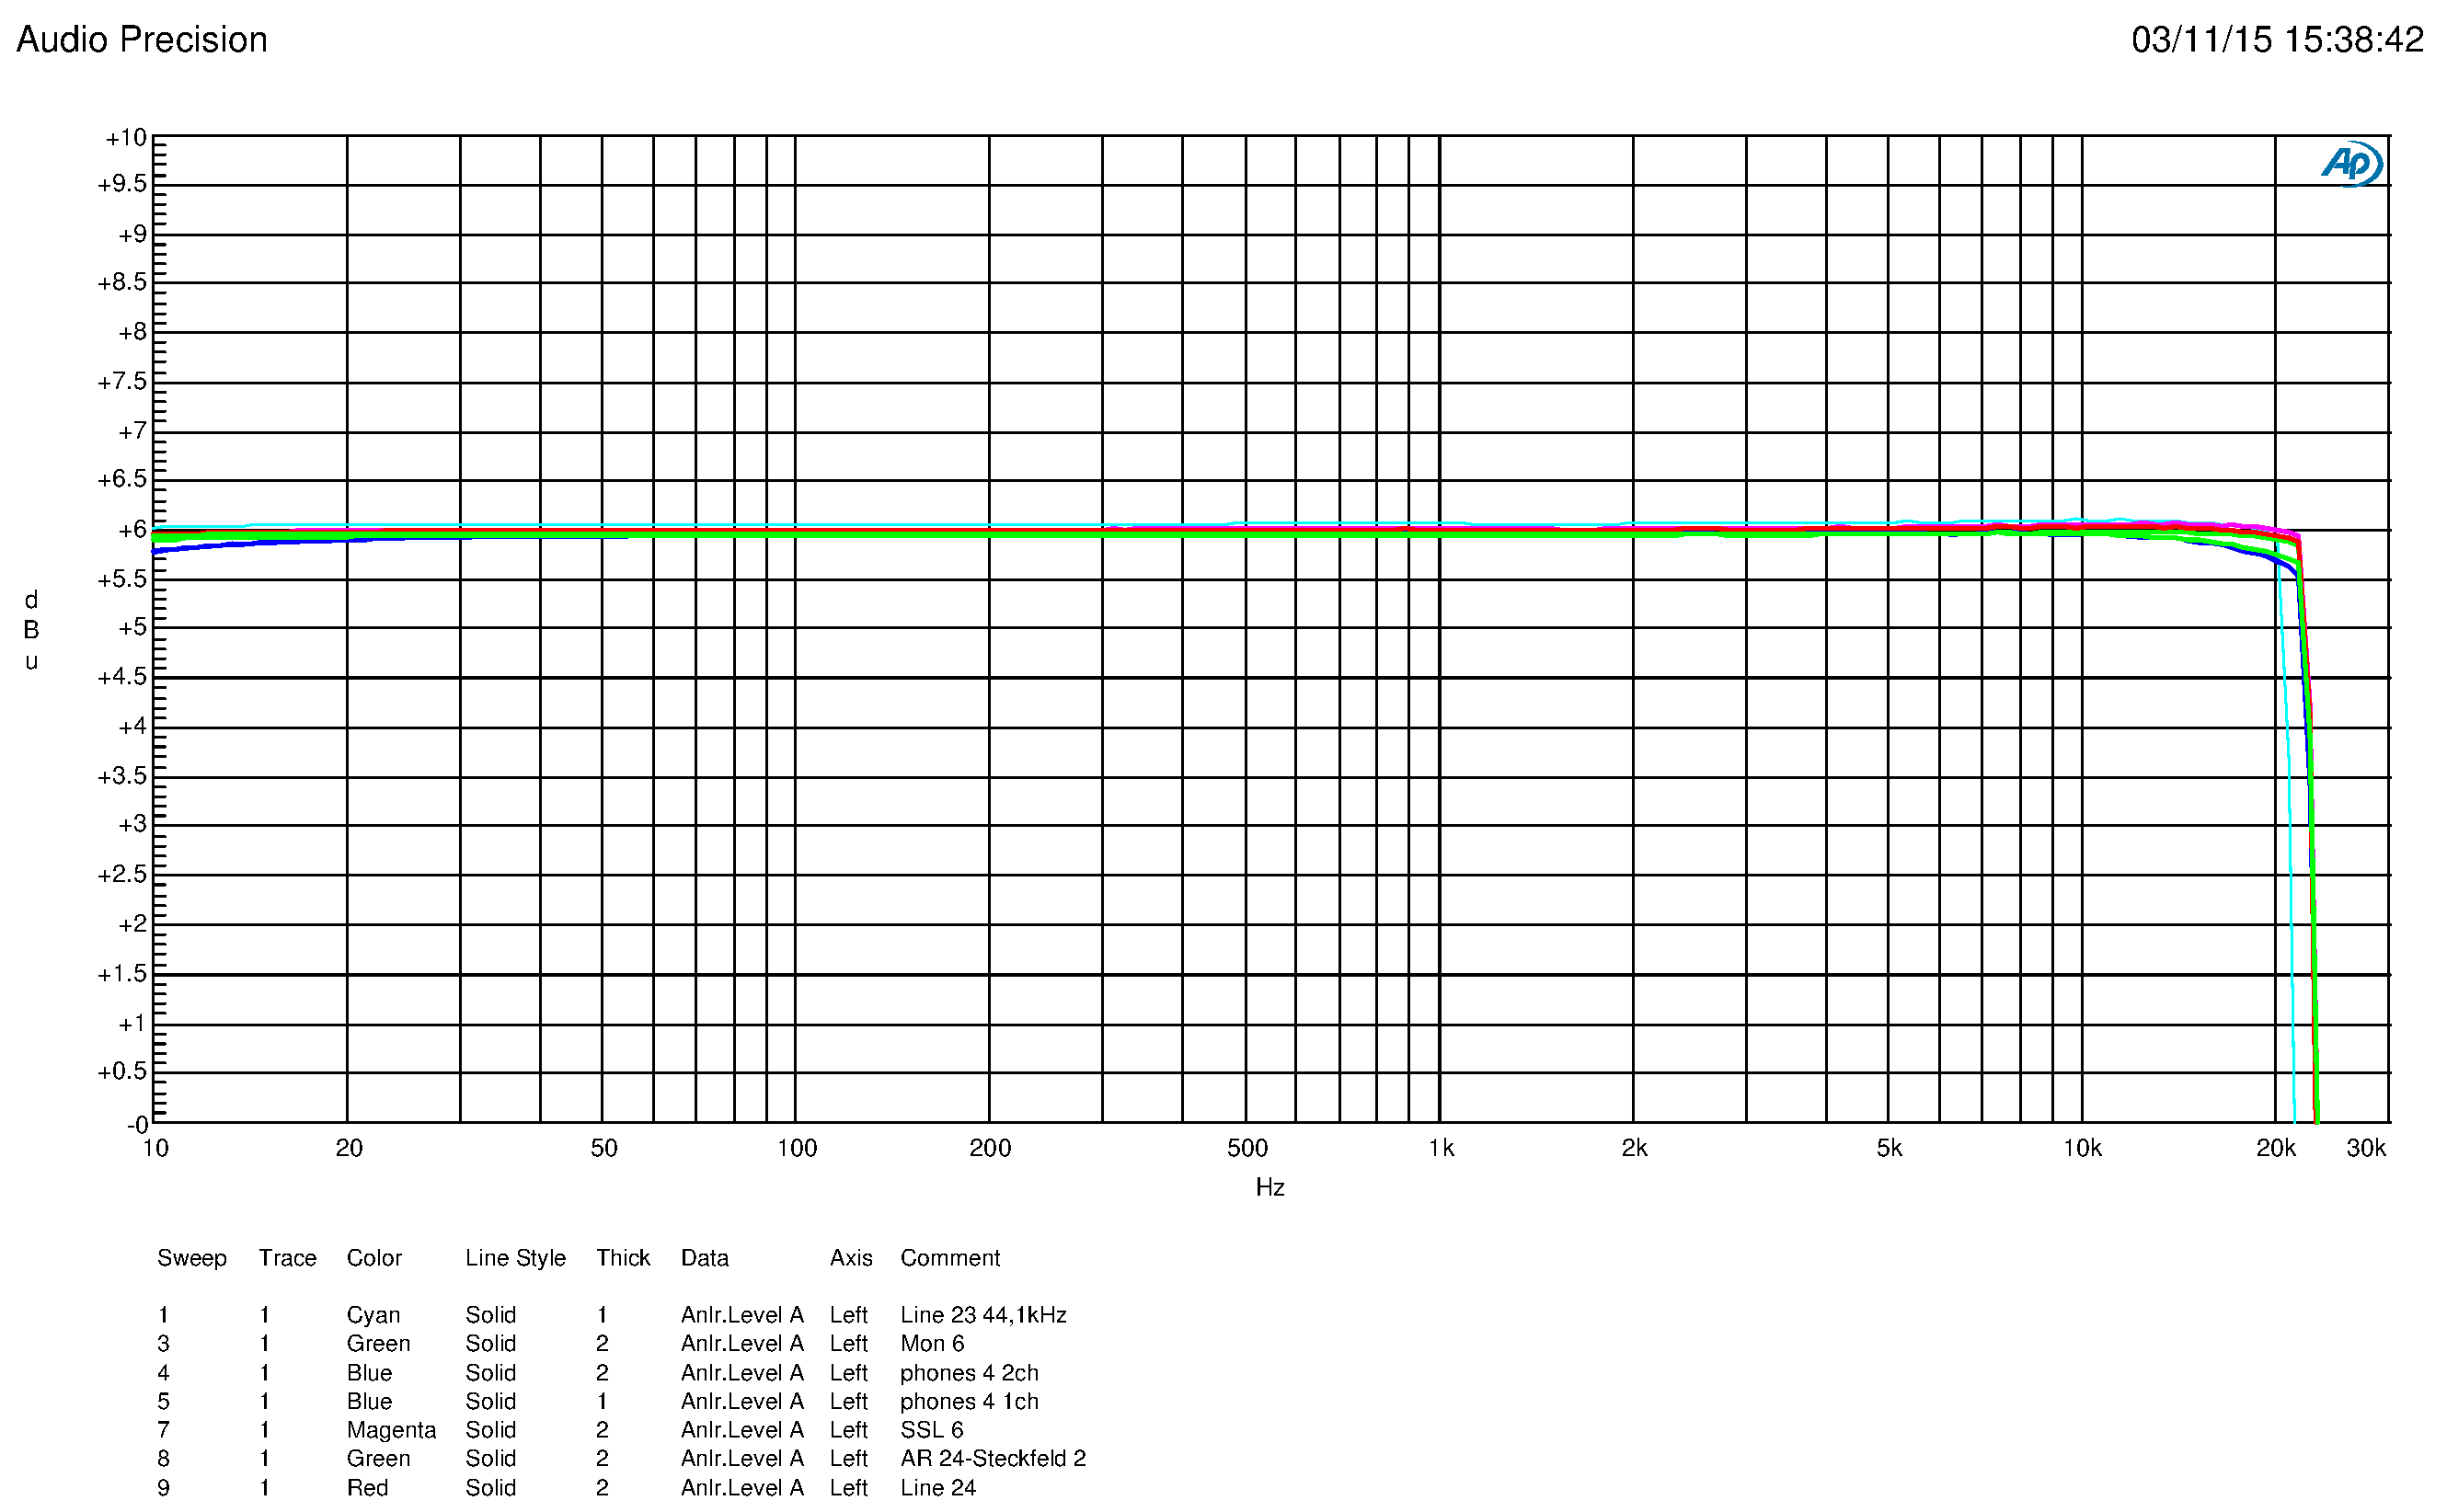
\includegraphics[width=14cm,keepaspectratio=true]{DAWandlerVergleich10dB}
\caption{frequency responses of different DACs}
\label{Abb.:1}
\end{center}
\end{figure}

\begin{figure}[htbp]
\begin{center}
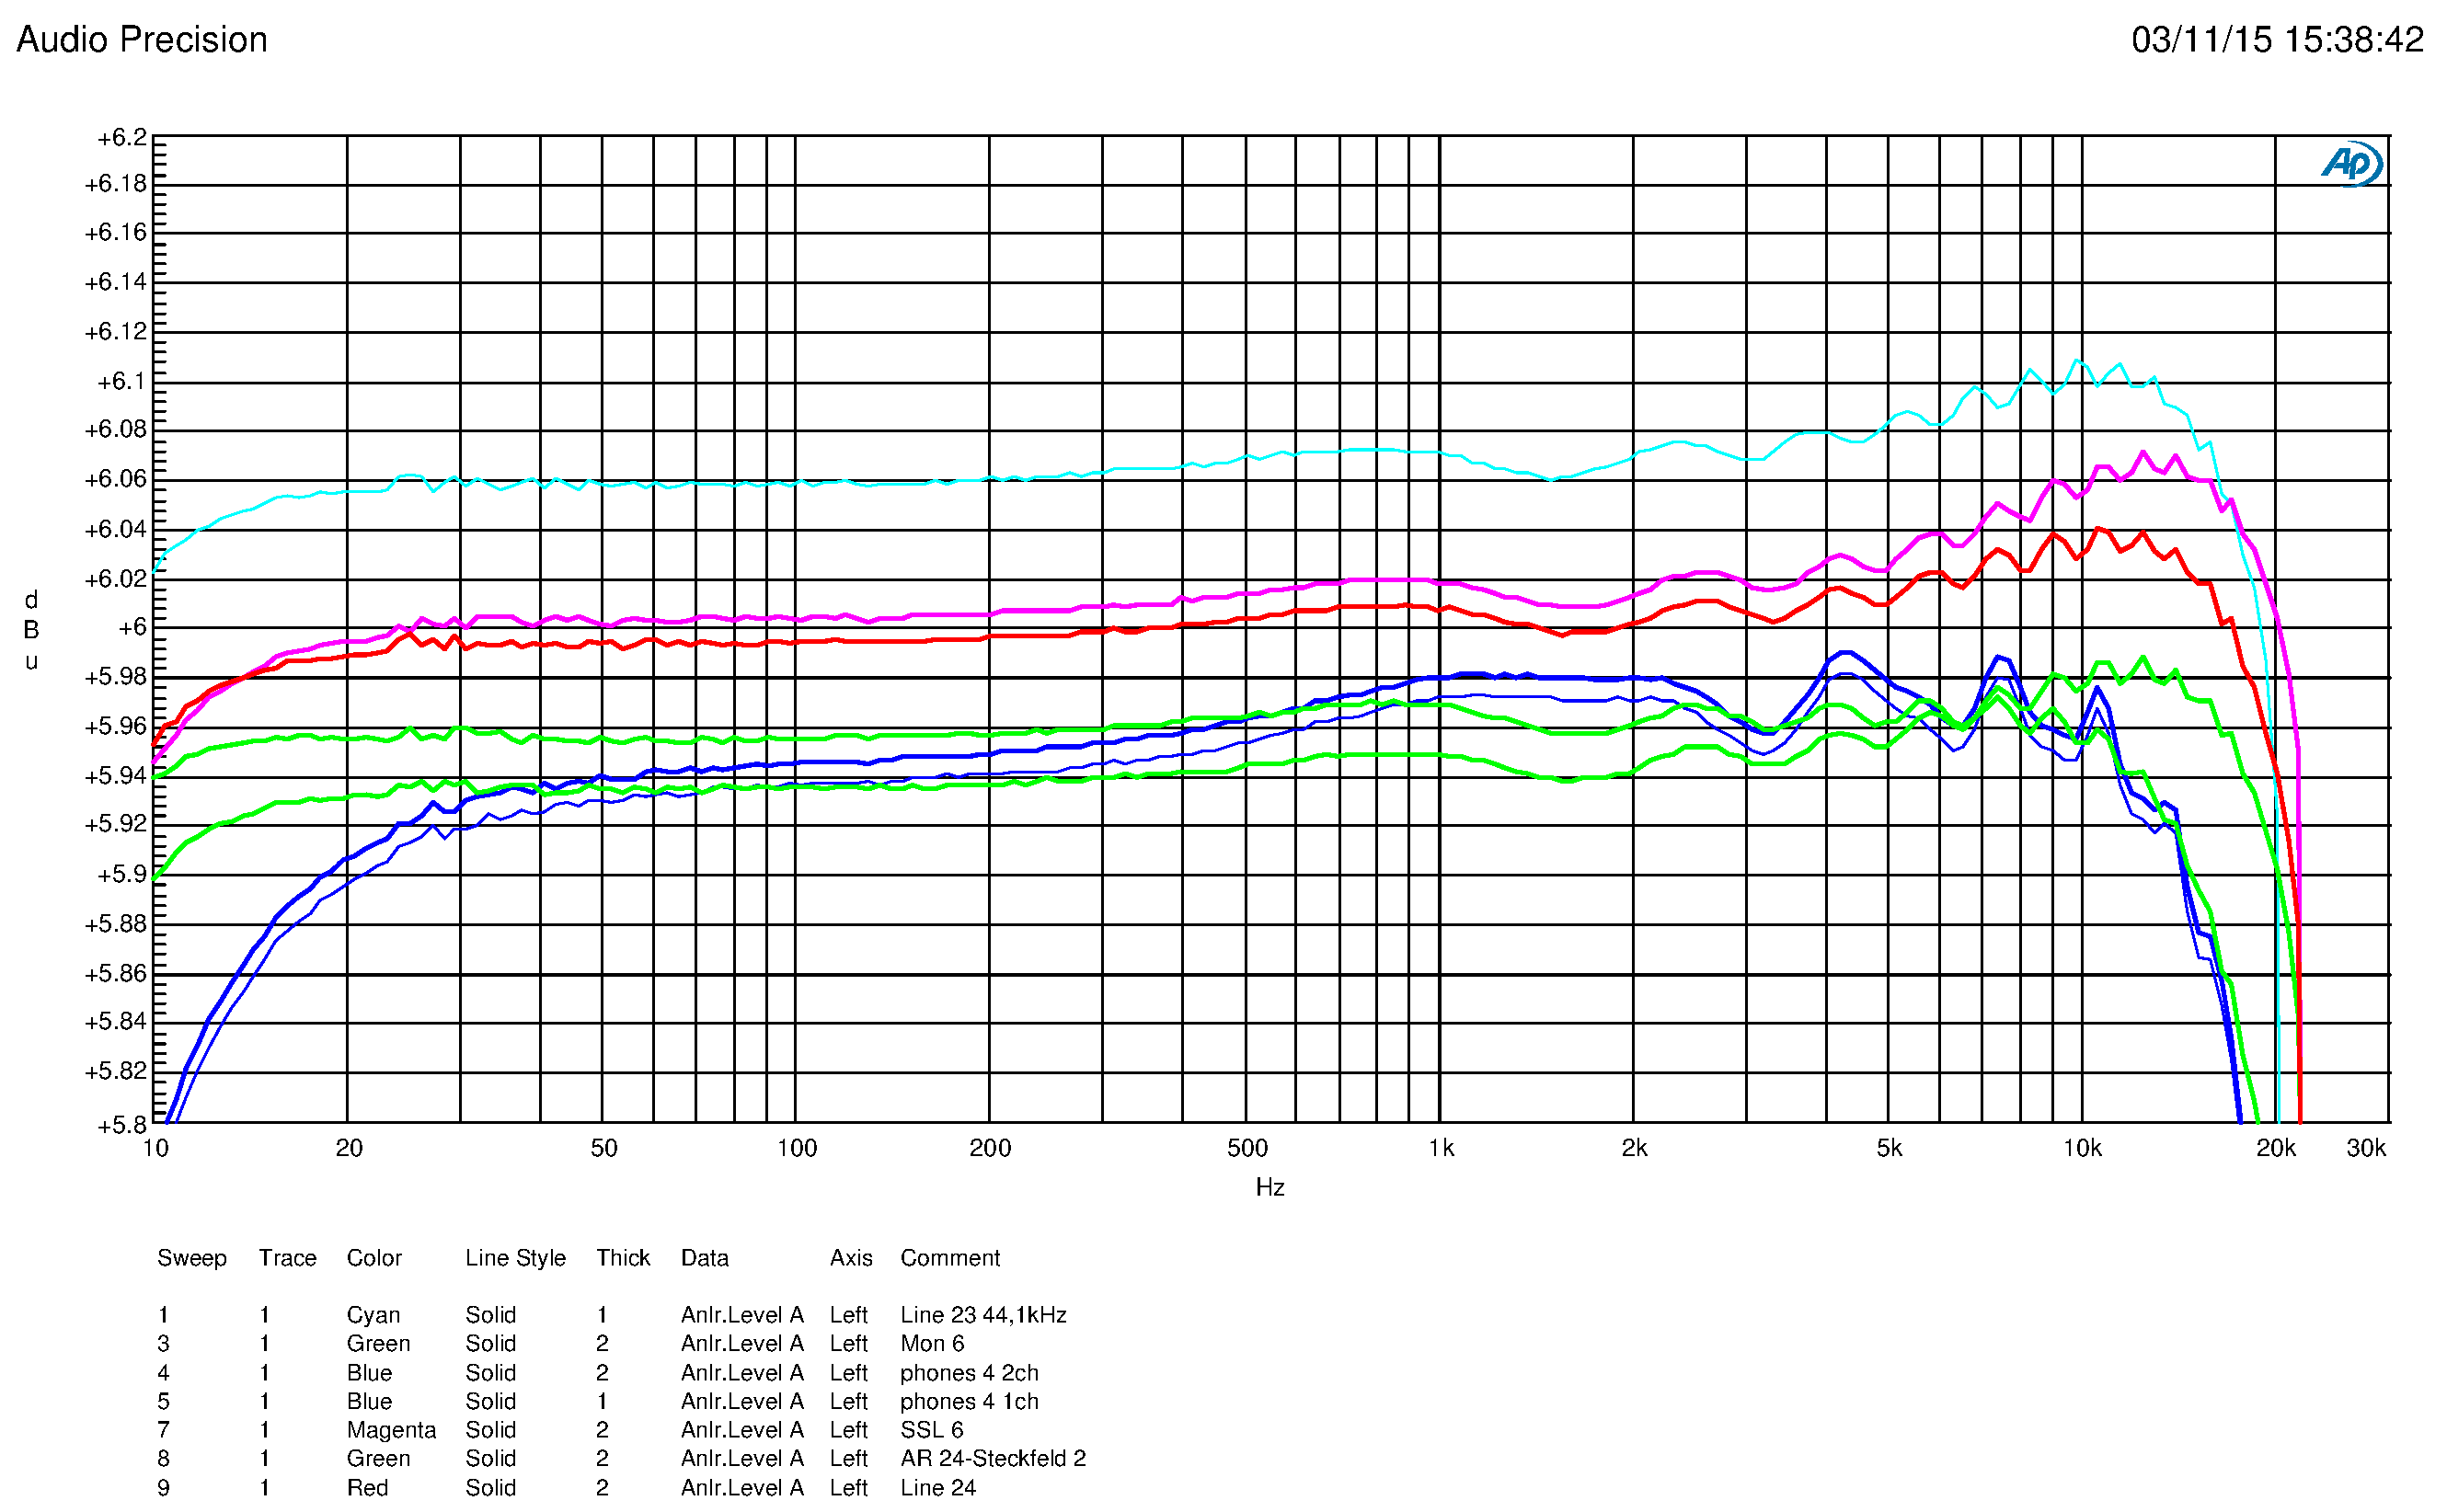
\includegraphics[width=14cm,keepaspectratio=true]{DaWandlerVergleich}
\caption{detailed frequency responses of different DACs}
\label{Abb.:1}
\end{center}
\end{figure}

\begin{figure}[htbp]
\begin{center}
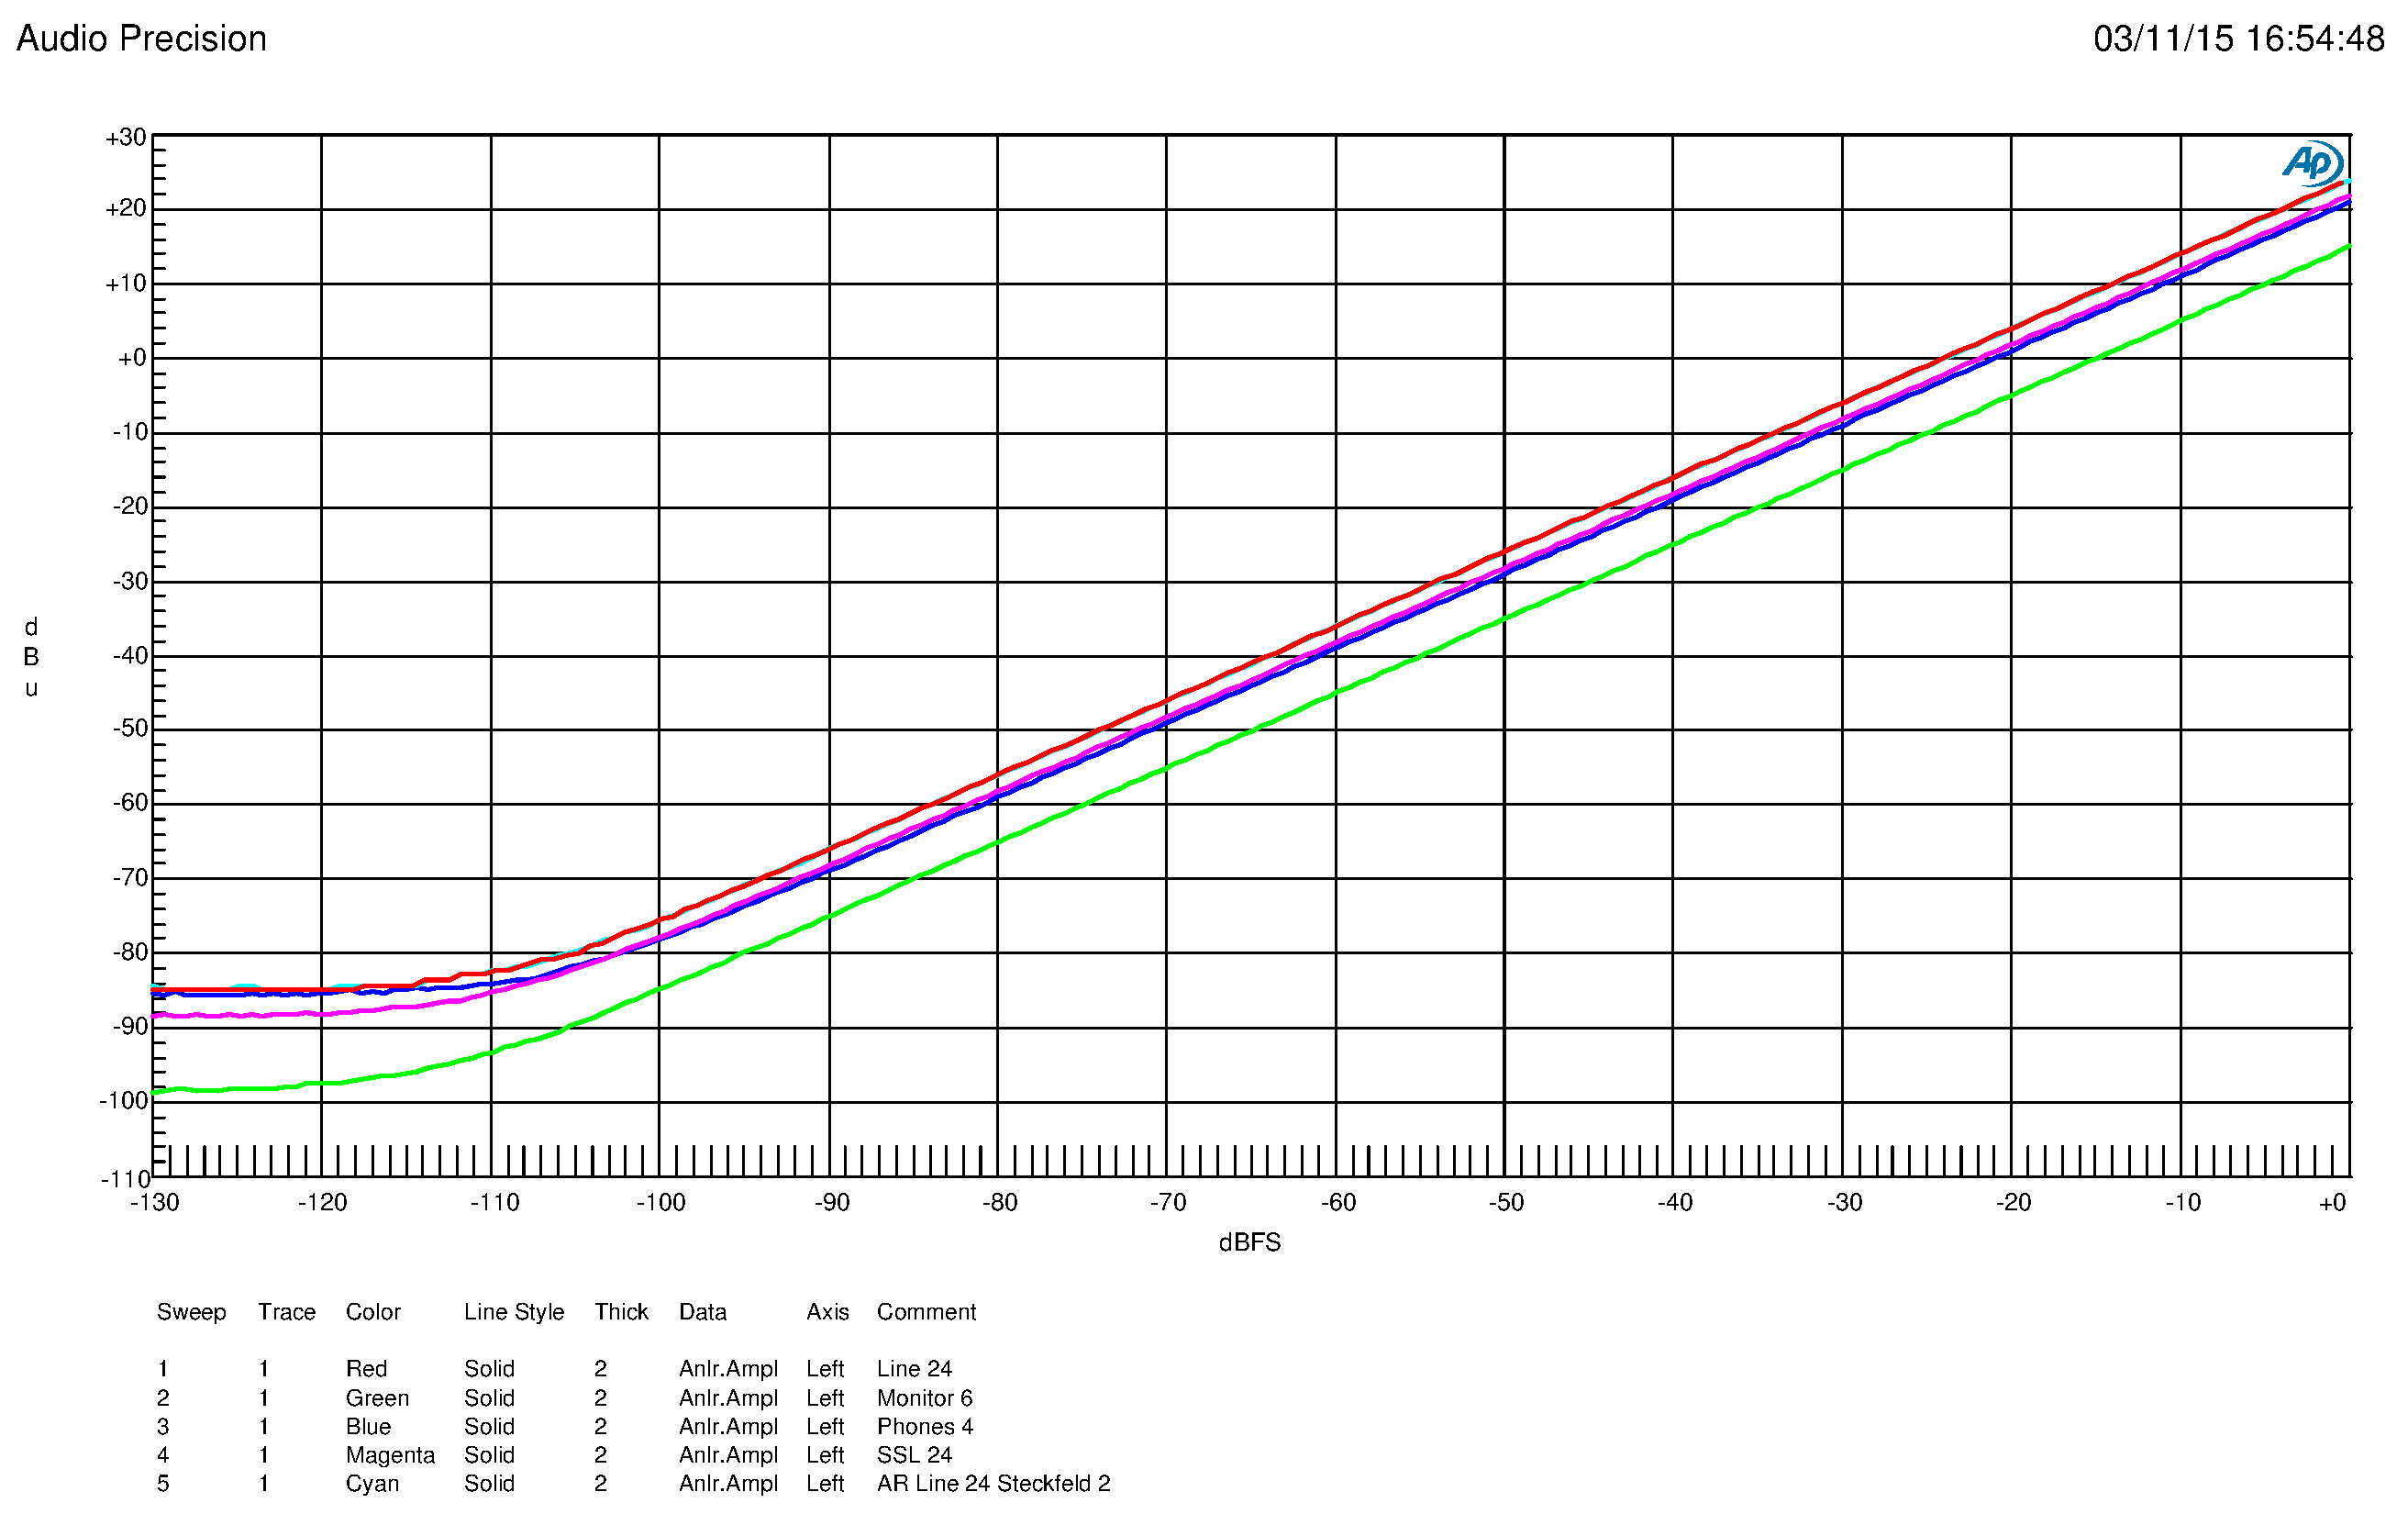
\includegraphics[width=14cm,keepaspectratio=true]{Dynamikvergleich}
\caption{dynamic ranges of different DACs}
\label{Abb.:1}
\end{center}
\end{figure}

\begin{figure}[htbp]
\begin{center}
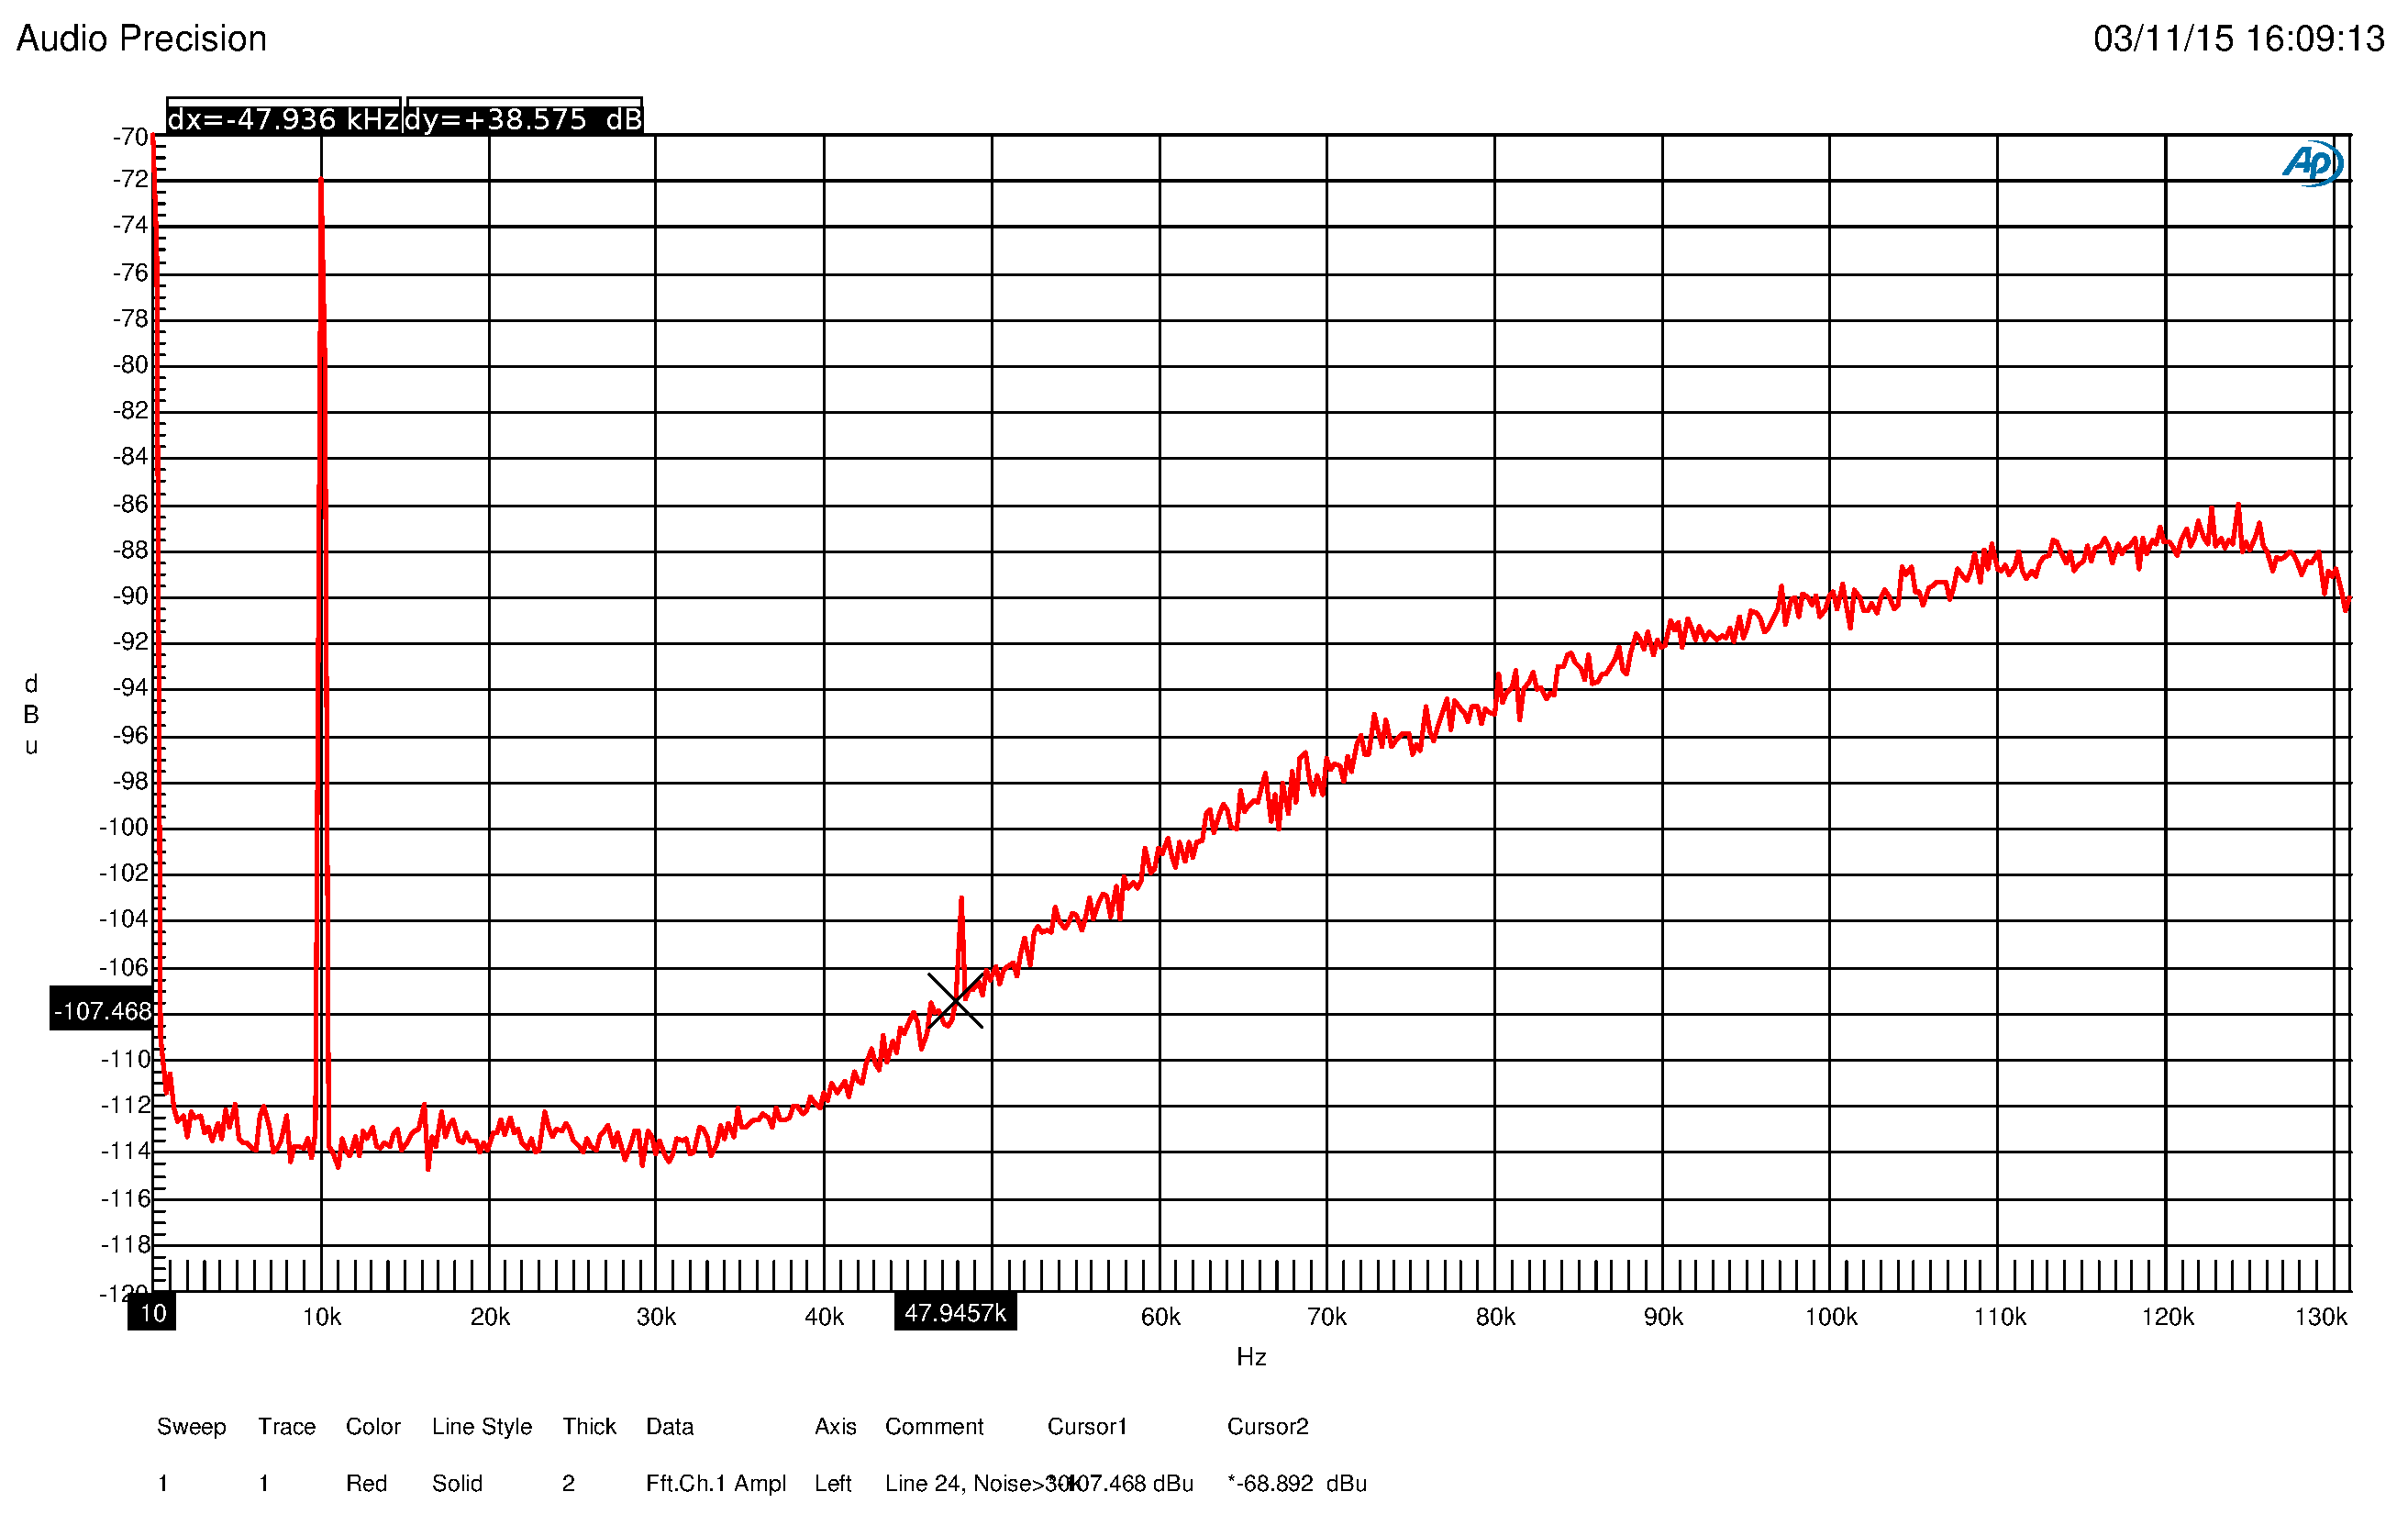
\includegraphics[width=14cm,keepaspectratio=true]{FFTrauschen}
\caption{FFT of line24 signal}
\label{Abb.:1}
\end{center}
\end{figure}

	\subsection{Discussion}


%---------------------------------------------------------------------------------------------------------
%---------------------------------------------------------------------------------------------------------
\chapter{ADC/preamplifier measurements}
\section{Introduction}
\subsection{ADC}
An analog-digital-converter converts an analog signal to a digital signal by sampling at discrete times and quantization of the analog signal to discrete amplitudes. Some important parameters for ADC quality measurements are
\begin{itemize}
\item resolution\\
The resolution of an ADC measures the number of quantization steps. Each analog value is set to the nearest quantization step. The higher the resolution is, the higher is the accuracy of the signal in the digital domain.
\item sampling rate\\
This parameter describes the number of time steps per second for quantization. For higher rates the signal can be converted more often and represented with more accuracy.
\item sampling time\\
The sampling time is a parameter which defines the time between sampling at the analog input and providing the digital value at the digital output.
\item jitter\\
The jitter regarding to ADCs measures the time difference between the optimal sampling point and the actual sampling point. For high quality ADCs this parameter should be very low.
\end{itemize}
\subsubsection{Quantization}
Quantization is the process of mapping a continuous signal to a countable set of values. The simplest way to quantize a signal is to round the sampled value to the nearest digital amplitude. Figure \ref{fig:quantization}  shows the quantization process. At discrete time steps the value of the input signal is measured and rounded to the nearest discrete value (green and yellow curve). The difference between those two signals is called quantization error or quantization noise and is shown in the red curve. As it can be seen quantization is a lossy process. The maximum error of quantization is always half of the step size between two symbols. The dynamic of quantization increases with every bit with
\begin{equation}
dyn_{[dB]}=20\cdot log(2^Q) \approx 1.761 + 6.02\cdot Q [dB]
\end{equation}
$$Q....number\; of\; bits$$
\begin{figure}[htbp]
\begin{center}
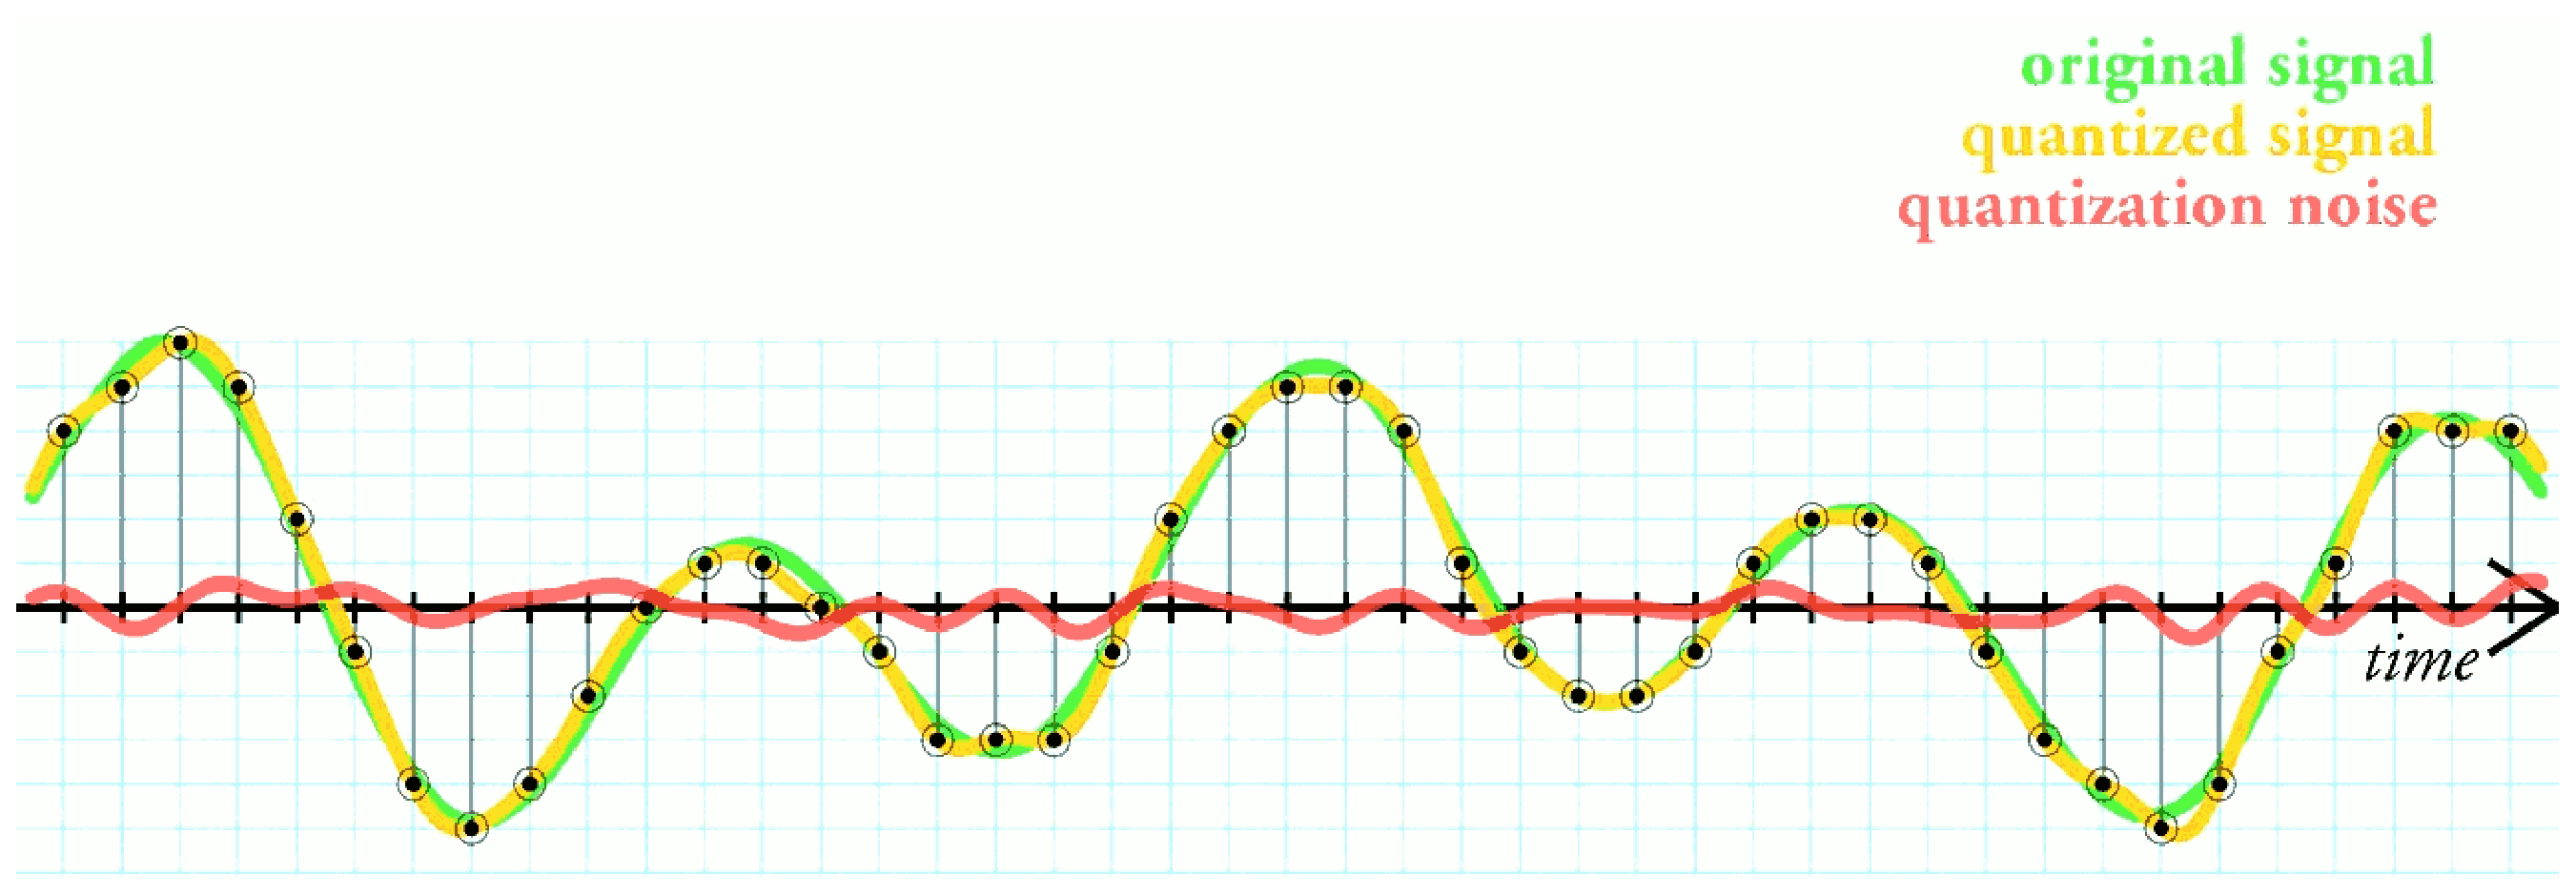
\includegraphics[width=14cm,keepaspectratio=true]{quantization}
\caption{analog-digital conversion of an analog signal}
\label{fig:quantization}
\end{center}
http://upload.wikimedia.org/wikipedia/commons/thumb/b/b8/Quantization\_error.png/500px-Quantization\_error.png
\end{figure}
At low amplitudes it can occur that the analog signal can not be quantized properly due to low resolution. In such case, additional dither can be used.
\subsubsection{Dithering}
Dithering describes the process of adding additional noise to a signal. In terms of audio engineering it helps to break up correlated error signals from quantization steps. Random noise is typially less objectionable than harmonic tones, produced by quantization. Dithering helps to break up those periodic cycles. Addionally noise shaping can be used. Noise energy at low frequency can be shaped and moved to higher frequency ranges, where the human listening is less affected.
\section{Measurements}
	\subsection{Experimental setup}
		\subsubsection{Equipment}
	\subsection{Results}
\begin{figure}[htbp]
\begin{center}
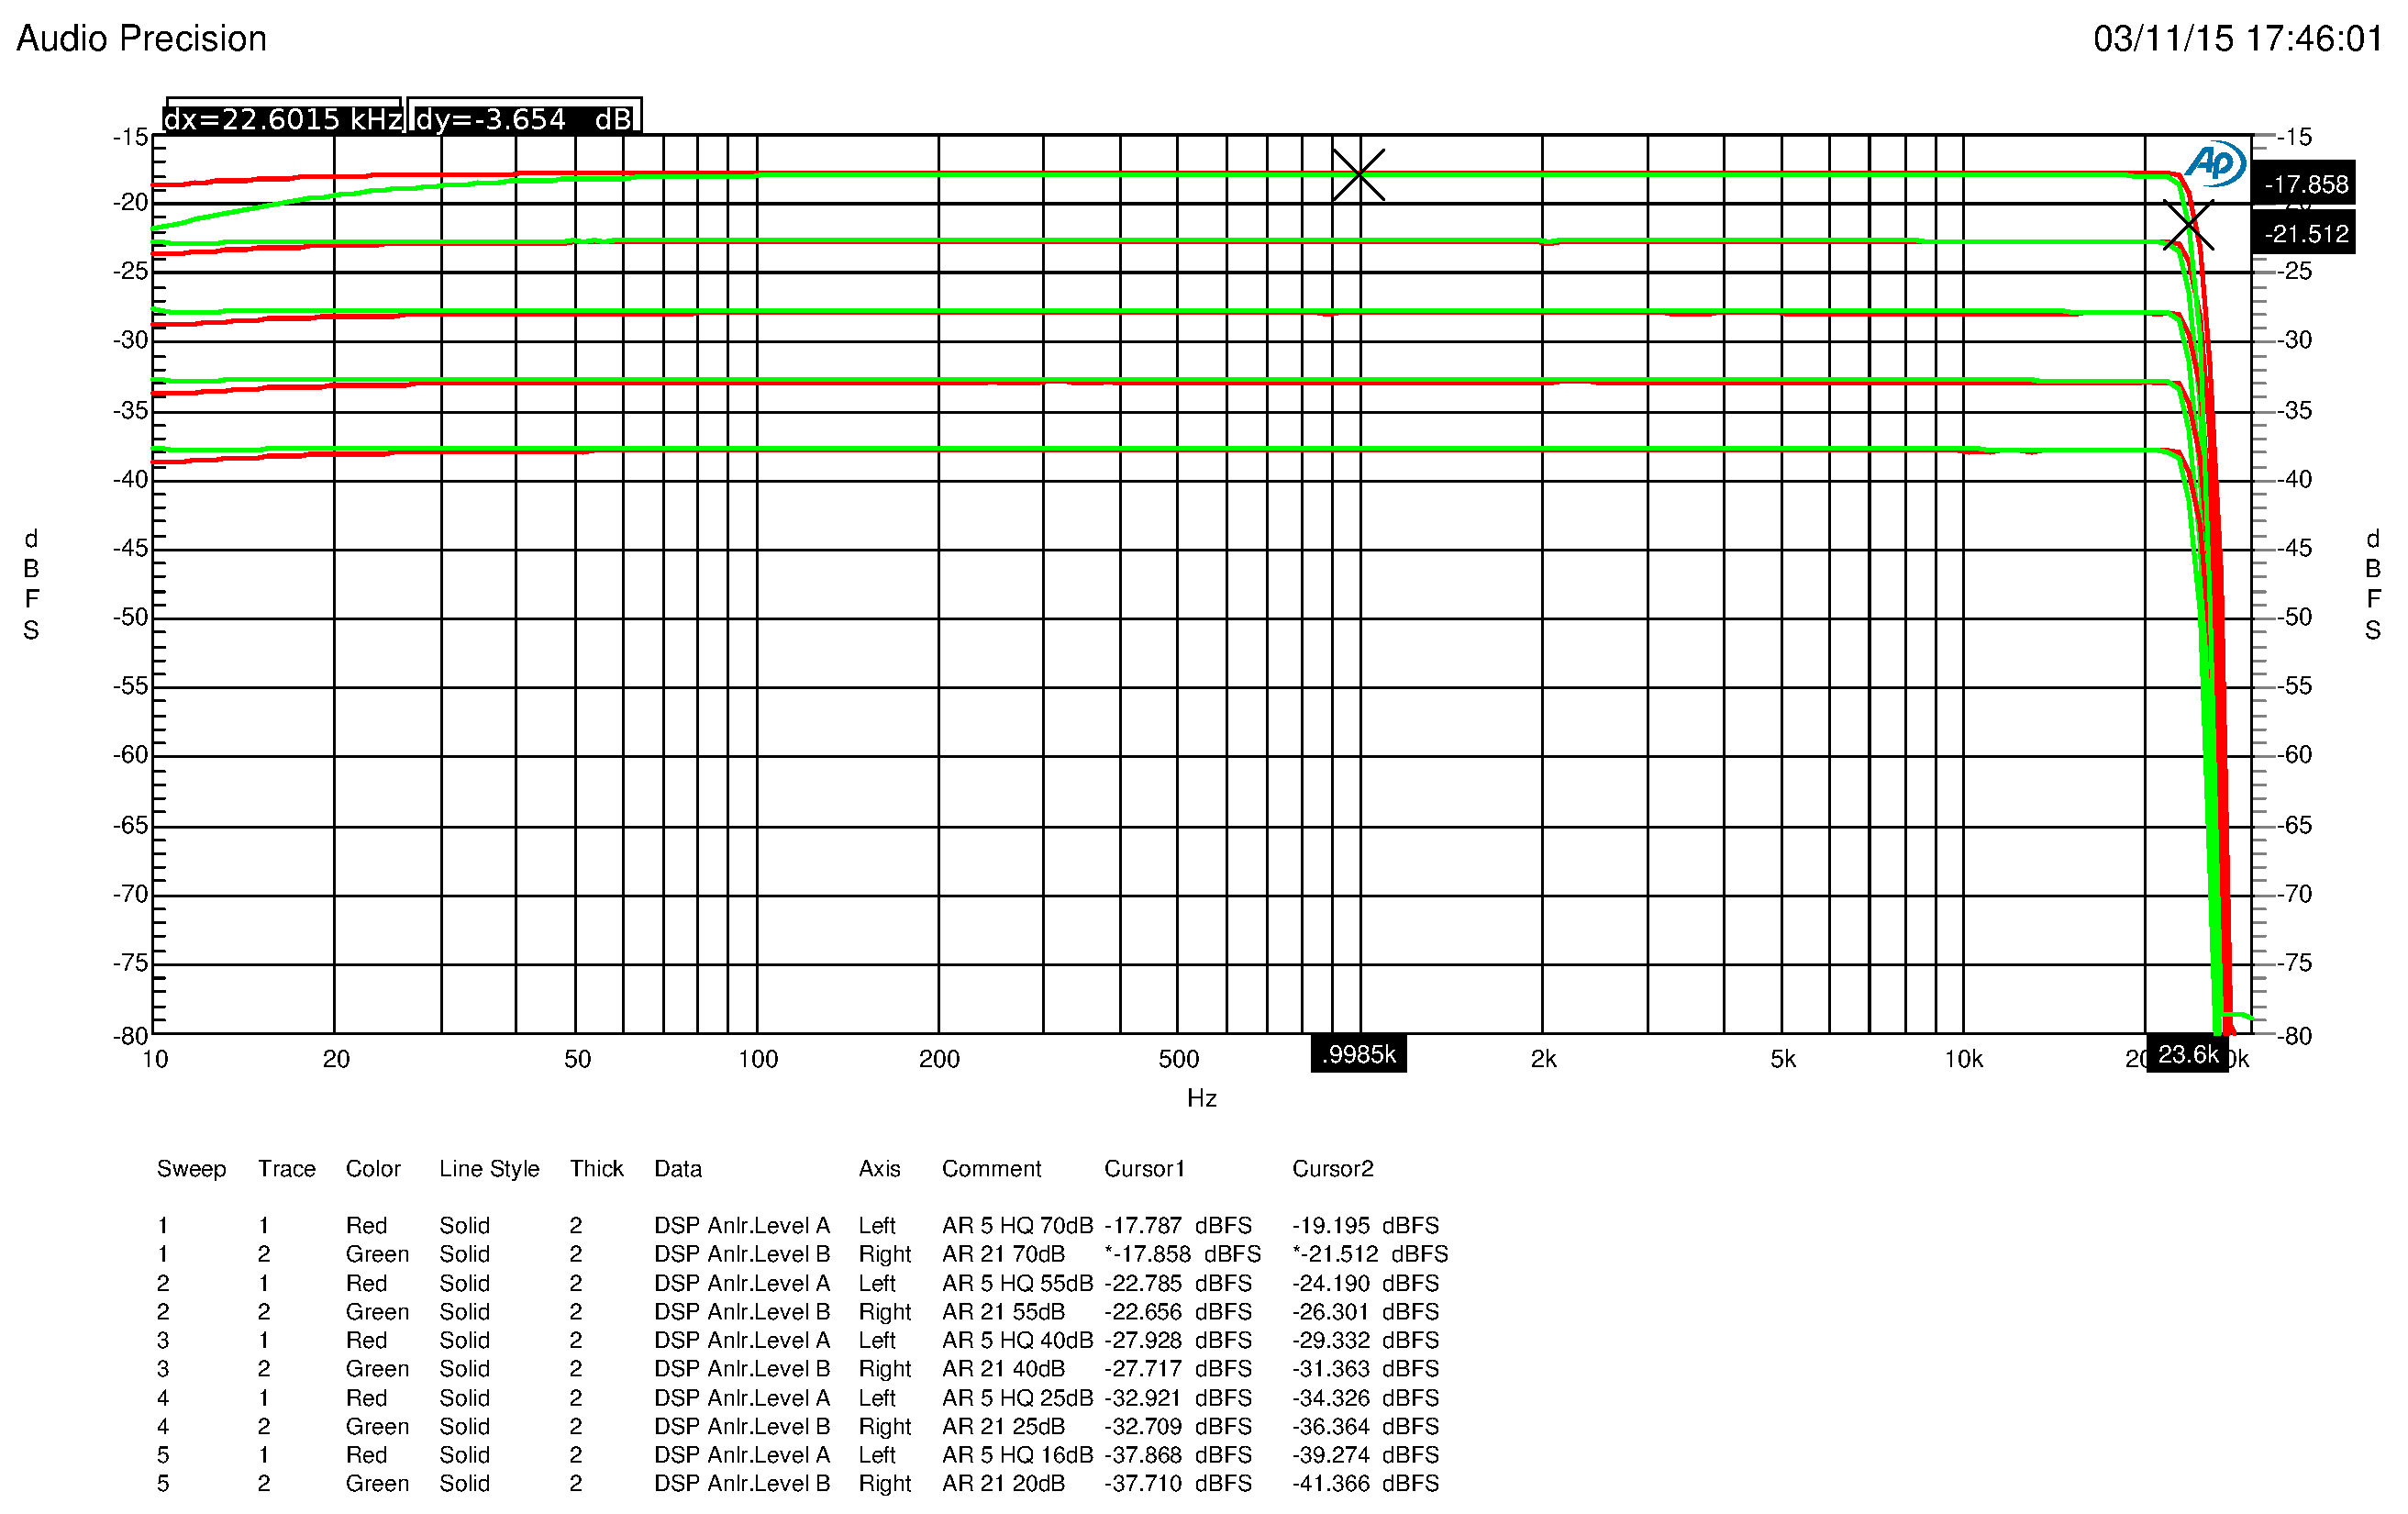
\includegraphics[width=14cm,keepaspectratio=true]{LAWOVorverstaerker5u21dB}
\caption{LAWO ADC and preamplifier}
\label{Abb.:1}
\end{center}
\end{figure}

\begin{figure}[htbp]
\begin{center}
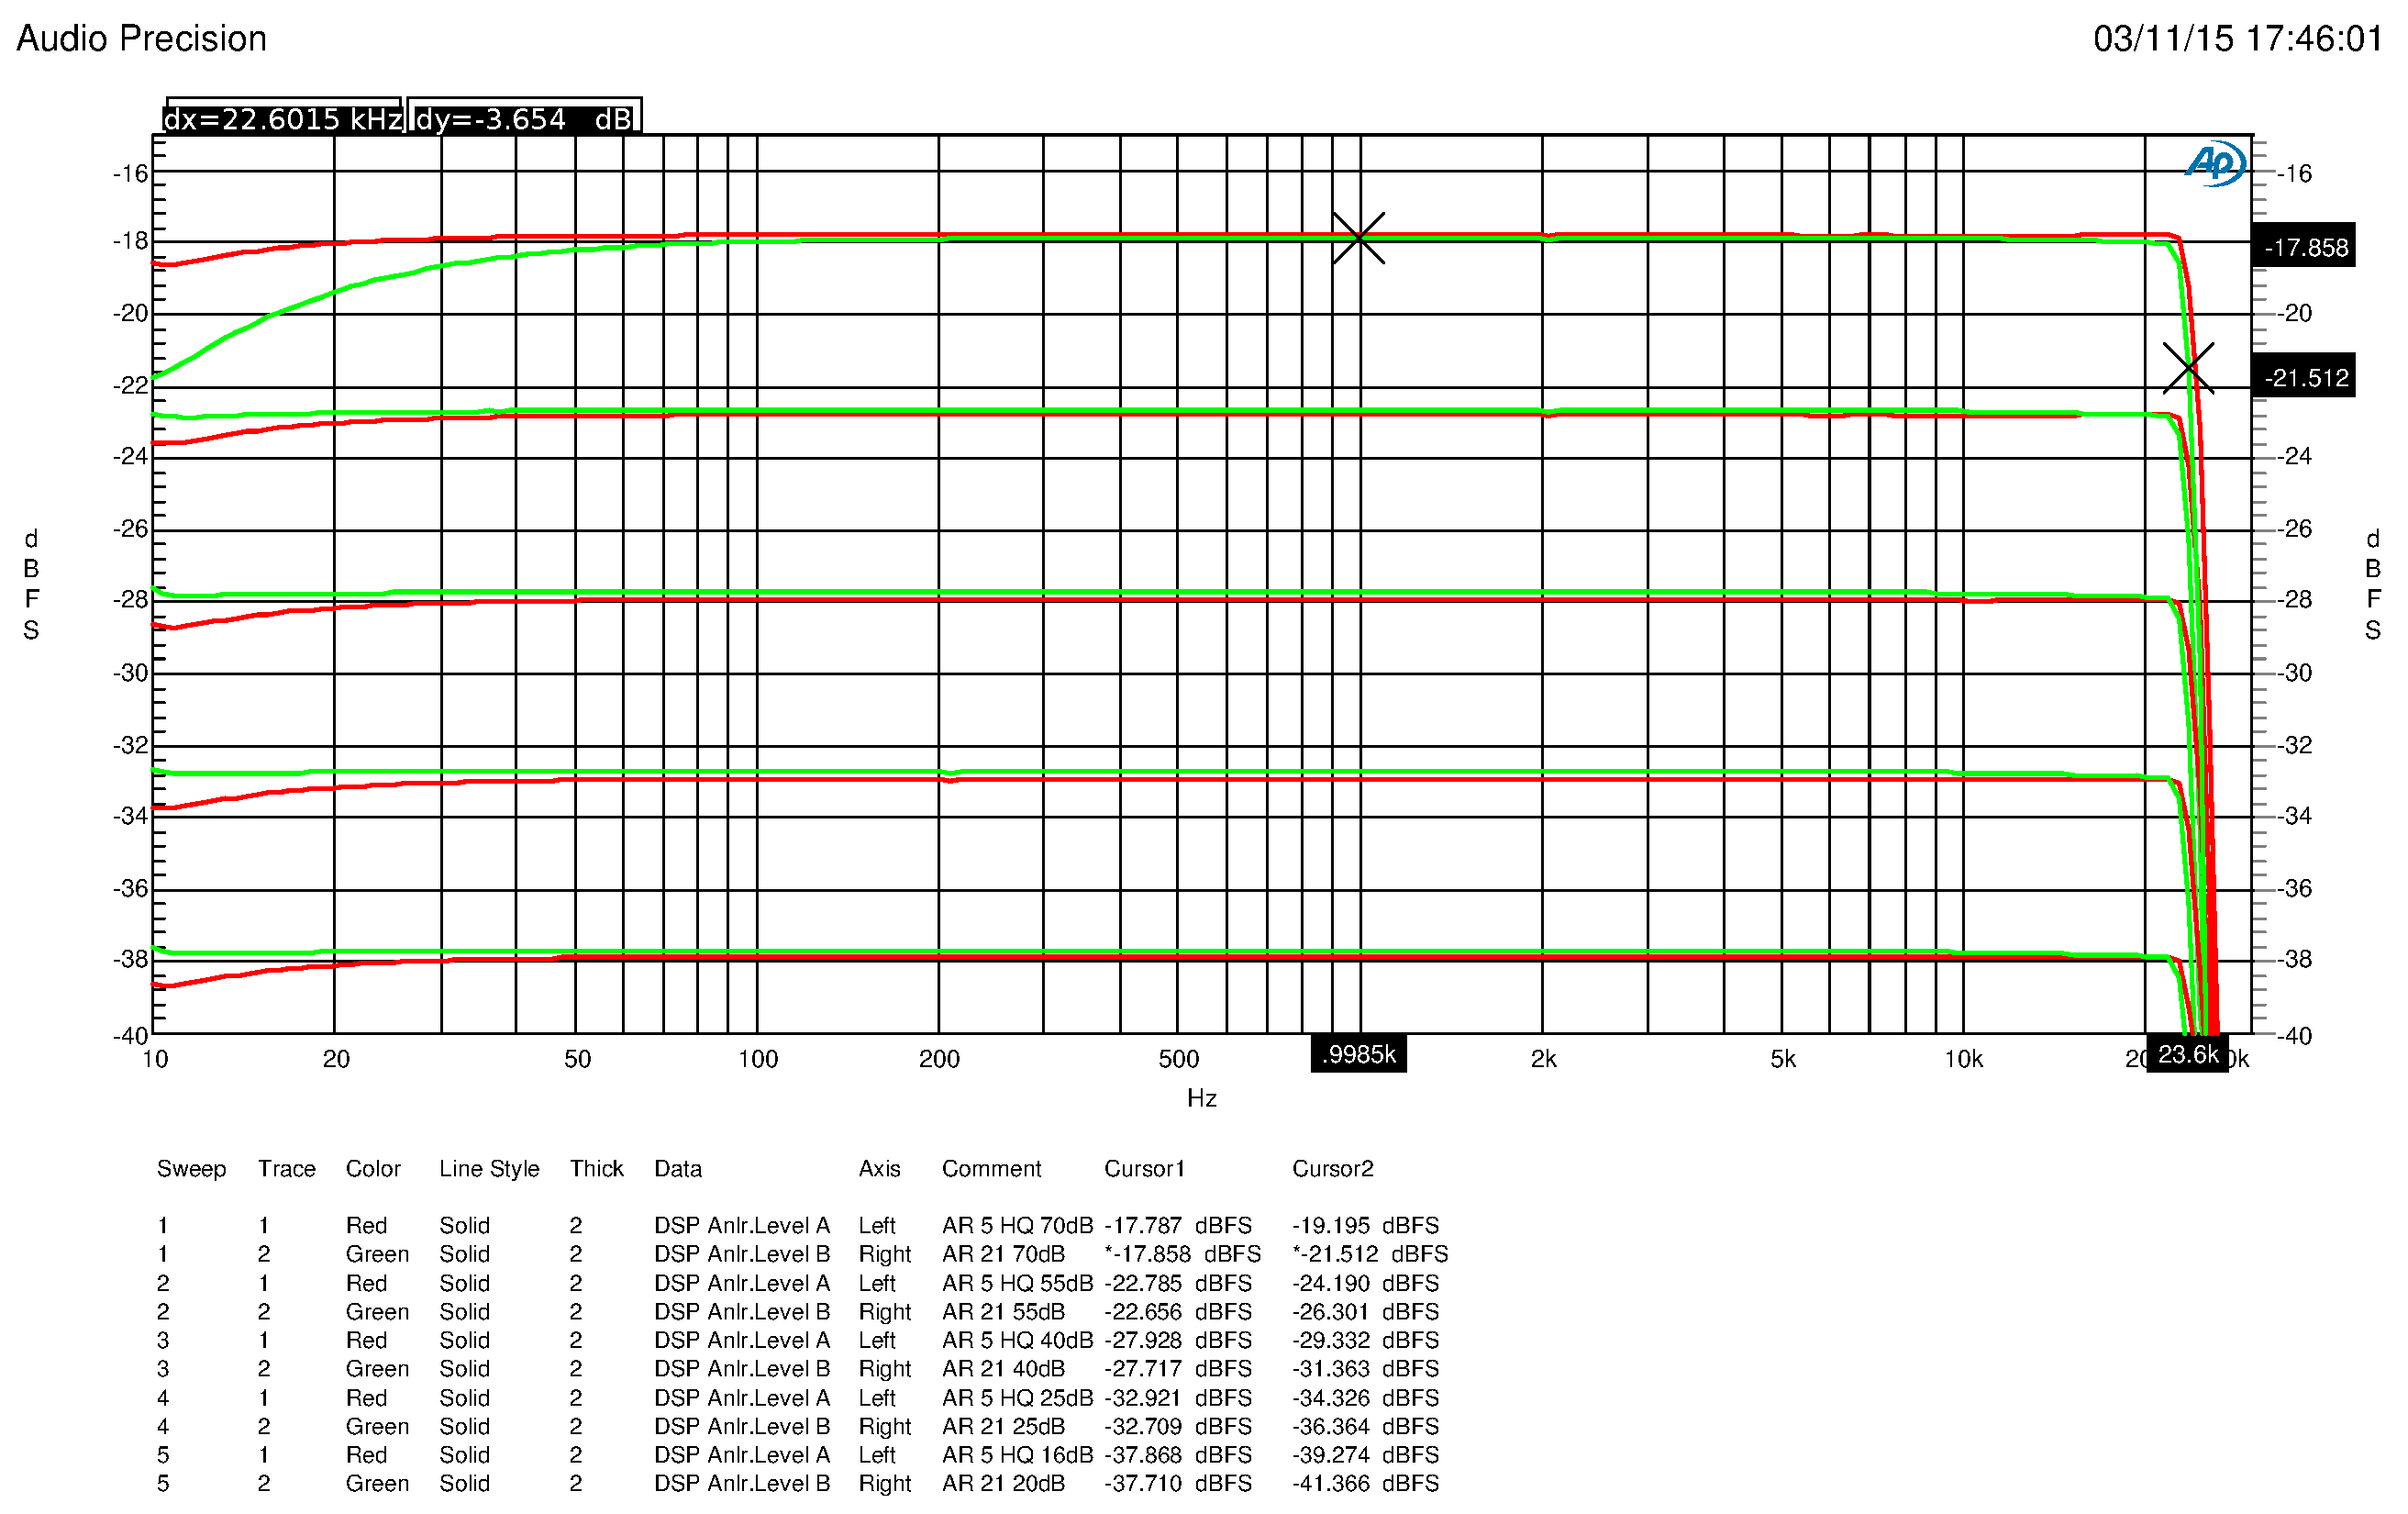
\includegraphics[width=14cm,keepaspectratio=true]{LAWOVorverstaerker5u21dBVergleichszoom}
\caption{LAWO ADC and preamplifier detailed view}
\label{Abb.:1}
\end{center}
\end{figure}

\begin{figure}[htbp]
\begin{center}
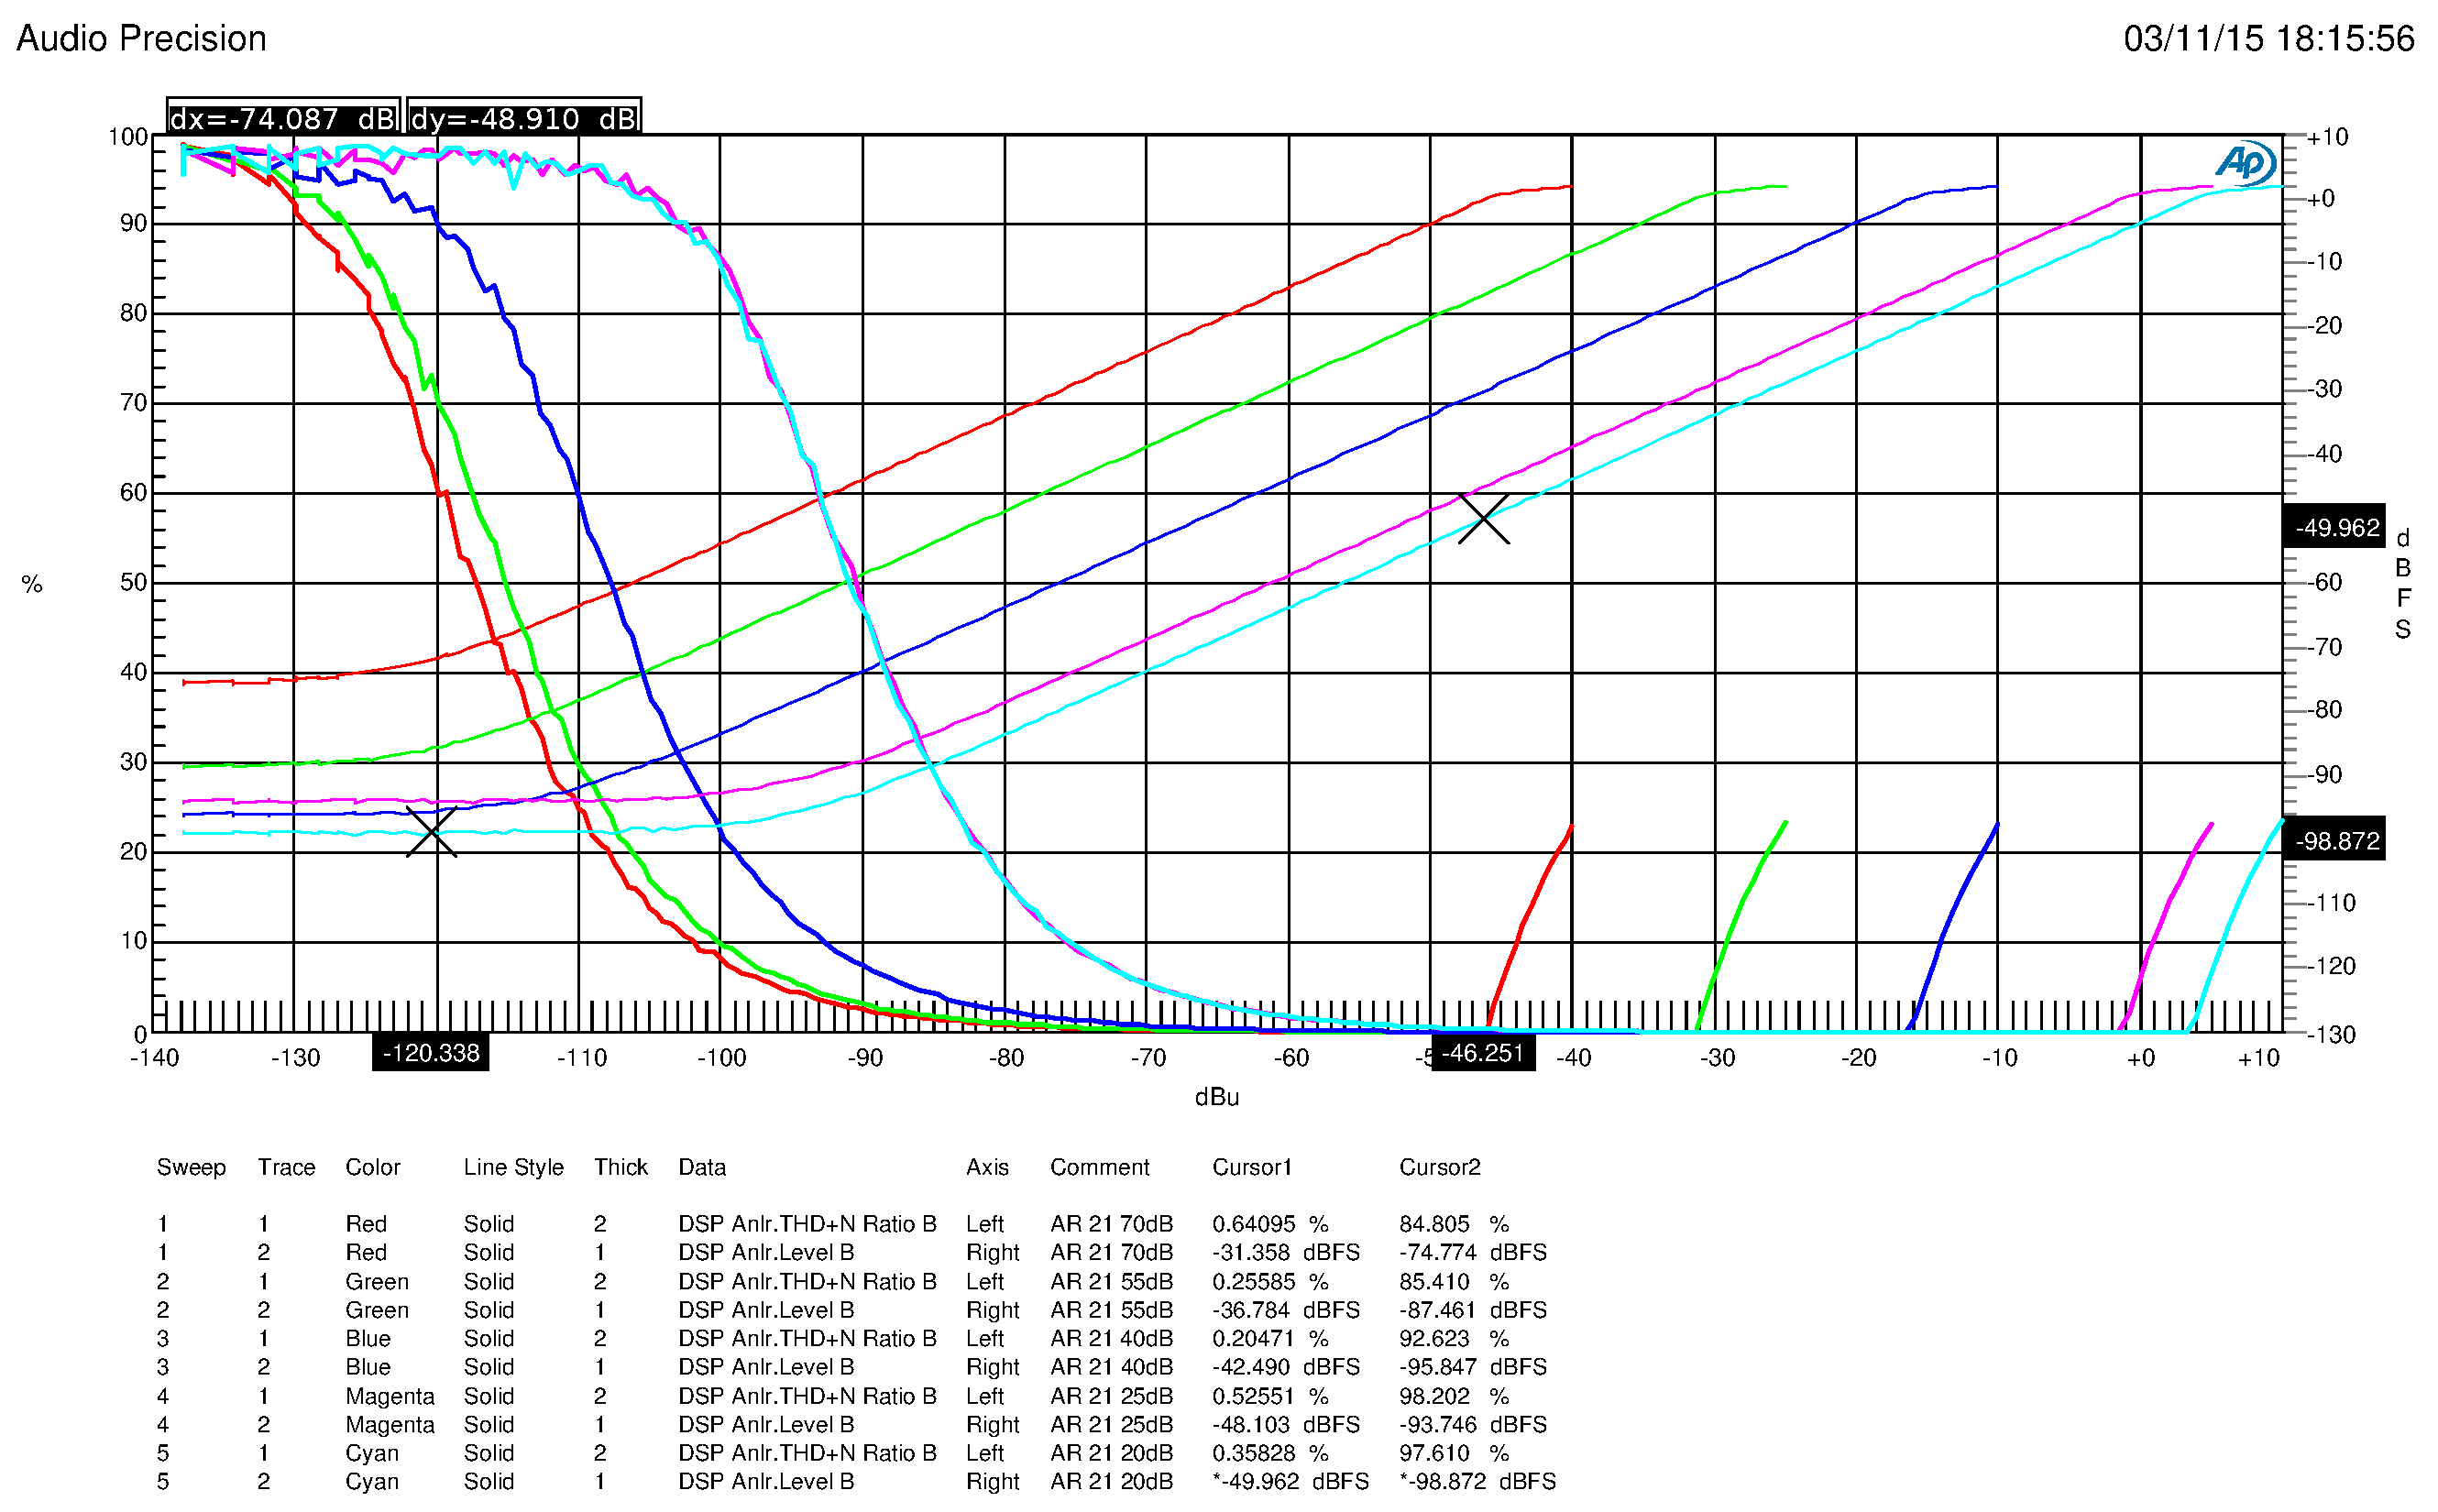
\includegraphics[width=14cm,keepaspectratio=true]{THDAR21dBVergleich}
\caption{dynamic range of channel AR21}
\label{Abb.:1}
\end{center}
\end{figure}

\begin{figure}[htbp]
\begin{center}
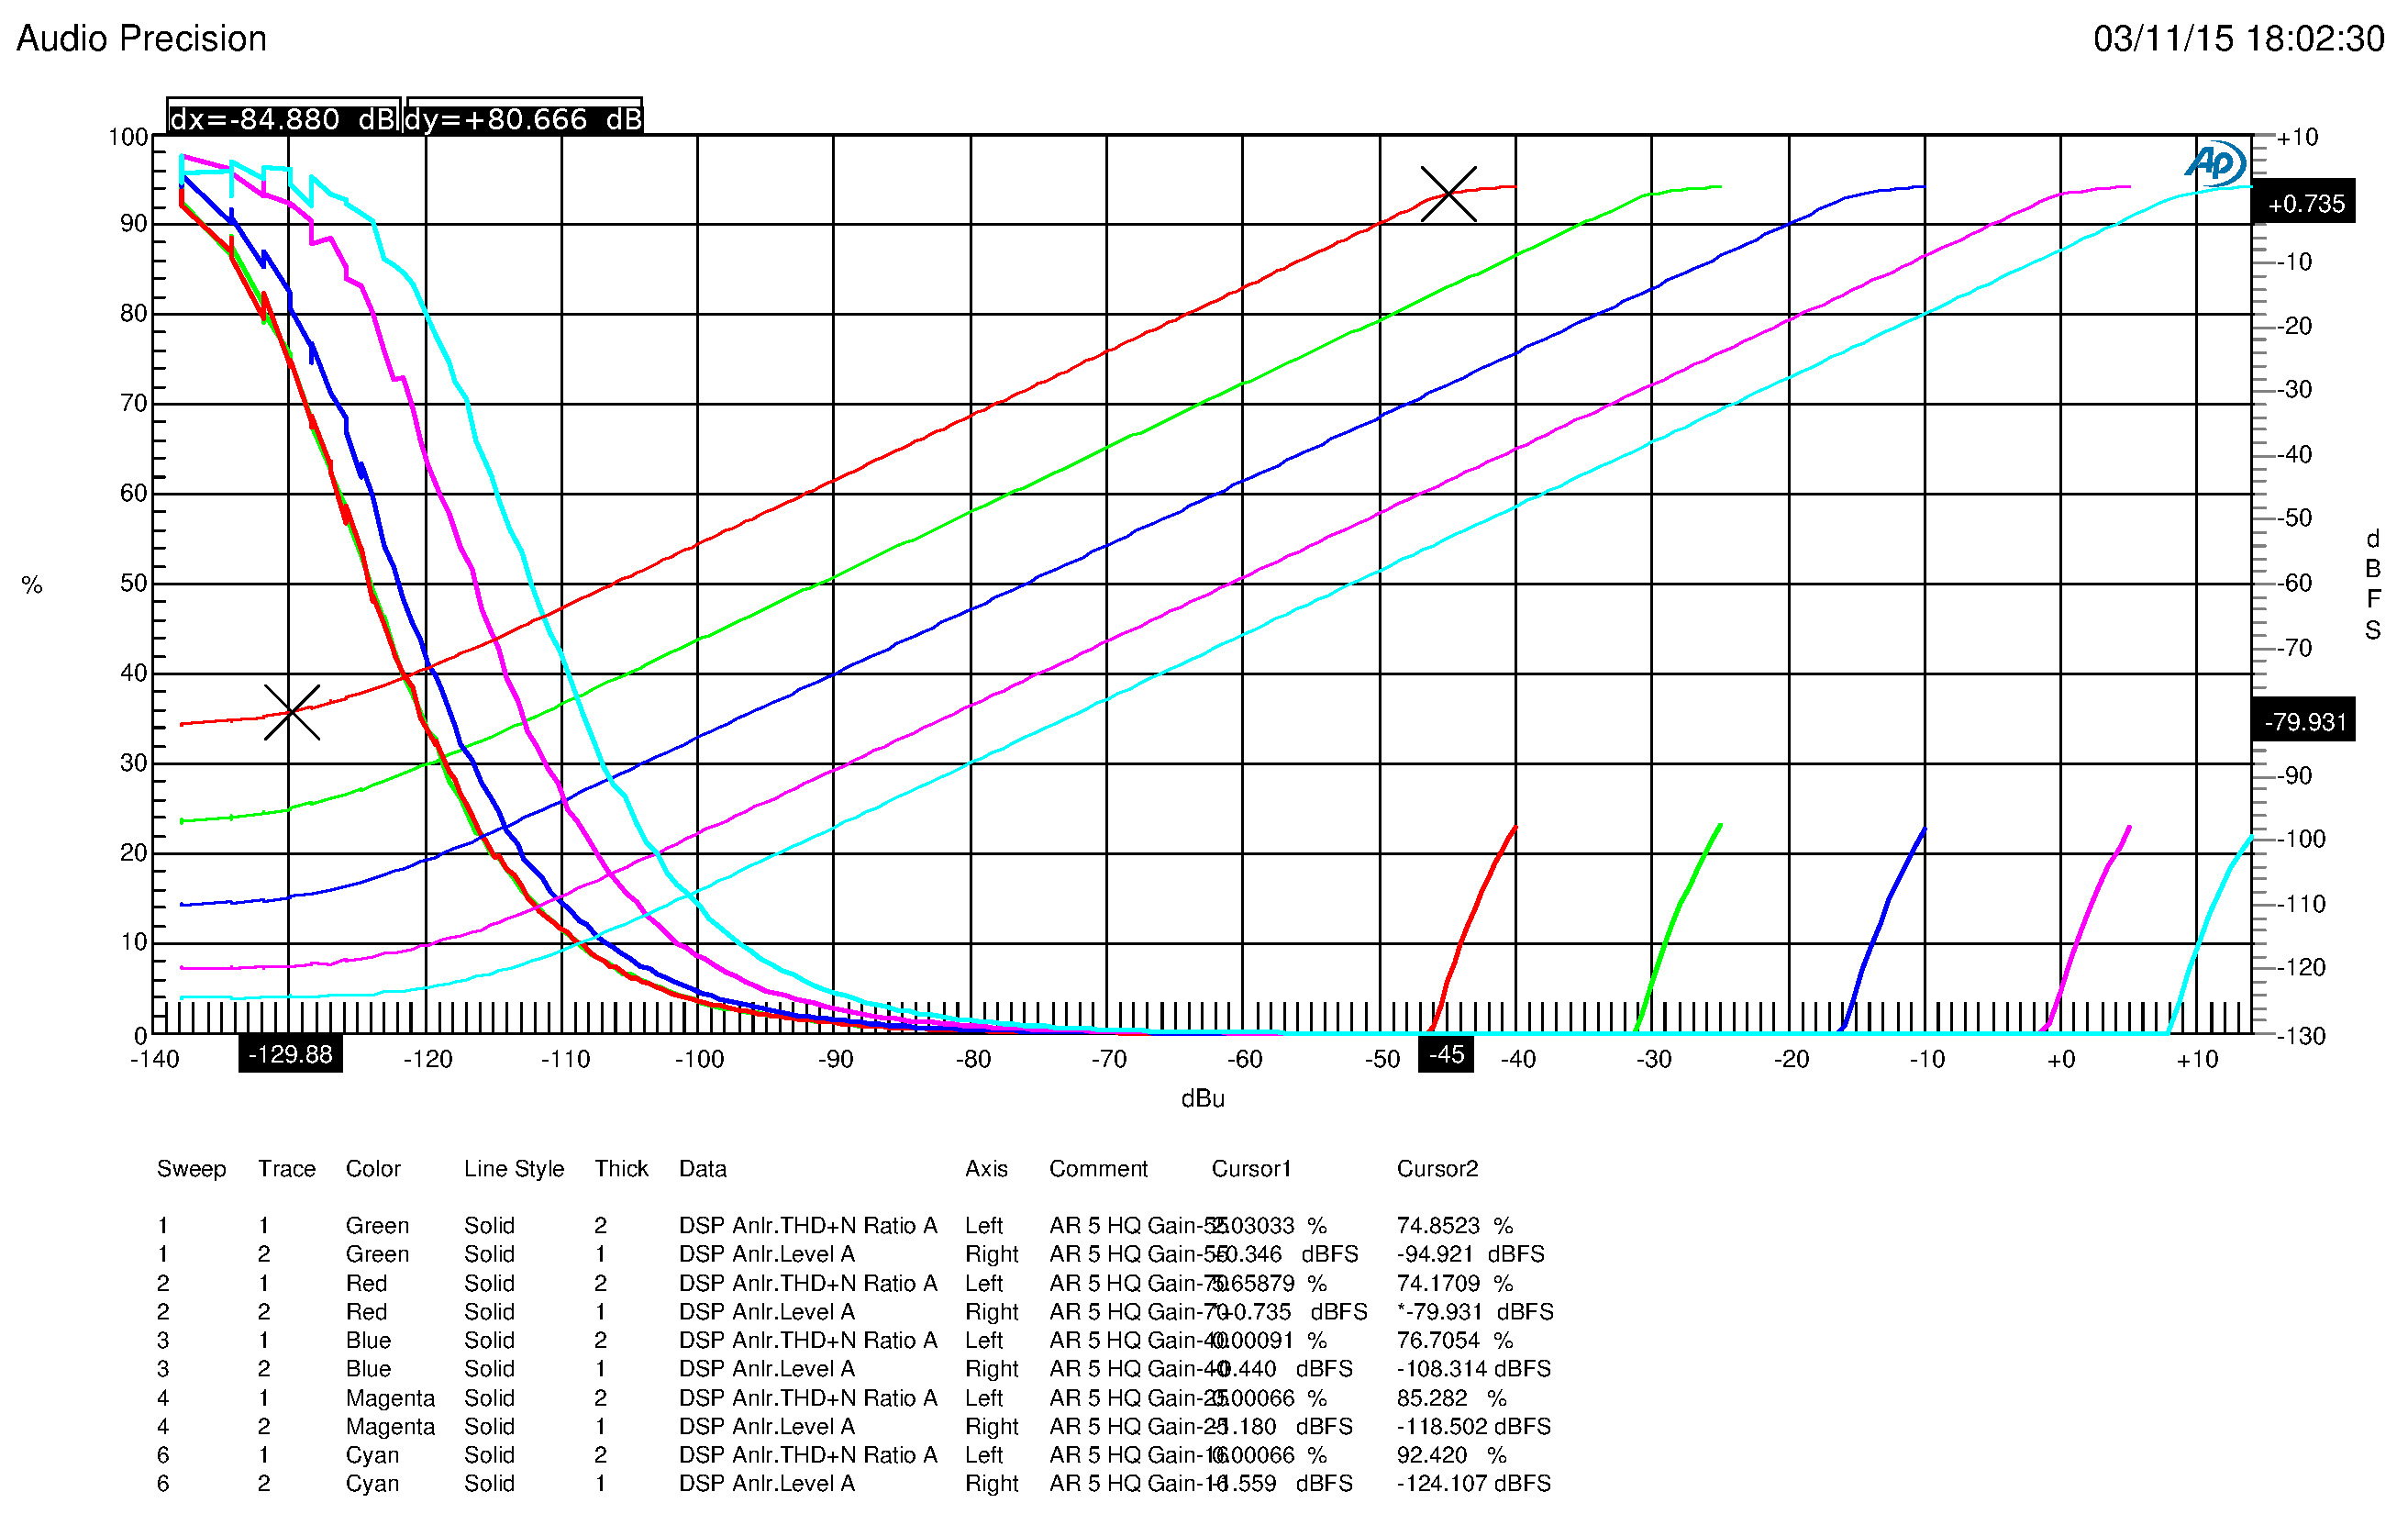
\includegraphics[width=14cm,keepaspectratio=true]{THDAR5HQdBVergleich}
\caption{dynamic range of high quality channel AR5}
\label{Abb.:1}
\end{center}
\end{figure}

	\subsection{Discussion}

%---------------------------------------------------------------------------------------------------------
%---------------------------------------------------------------------------------------------------------
\chapter{Conclusion}



\begin{center}
\begin{tabular}{|c||c|c|}
\hline 
SIL & 	PFH &		RRF\\ \hline
1 &	0.00001-0.000001 &	100,000-1,000,000\\
2 &	0.000001-0.0000001 &		1,000,000-10,000,000\\
3 &	0.0000001-0.00000001 		& 10,000,000-100,000,000\\
4 &	0.00000001-0.000000001 &	100,000,000-1,000,000,000\\
\hline
\end{tabular}
\end{center}


\begin{center}
\begin{figure}[htbp]
\includegraphics[width=11cm,keepaspectratio=true]{PROFIsafe}
\caption{PROFIsafe}
\label{Abb.:1}
\end{figure}
\end{center}


\begin{appendix}
\chapter{List of Abbreviations}
\nomenclature{ADC}{analog to digital converter}
\nomenclature{DAC}{digital to analog converter}
\nomenclature{THD}{total harmonic distortion}
\nomenclature{THD+N}{total harmonic distortion including noise}
\nomenclature{HQ}{high quality}
\nomenclature{AP}{AudioPrecision}
\nomenclature{AR}{Aufnahmeraum, audio studio TU Graz}
\nomenclature{RP1}{Regieplatz 1, audio studio TU Graz}
\printnomenclature


\chapter{High resolution diagrams}
\begin{figure}[htbp]
\begin{center}
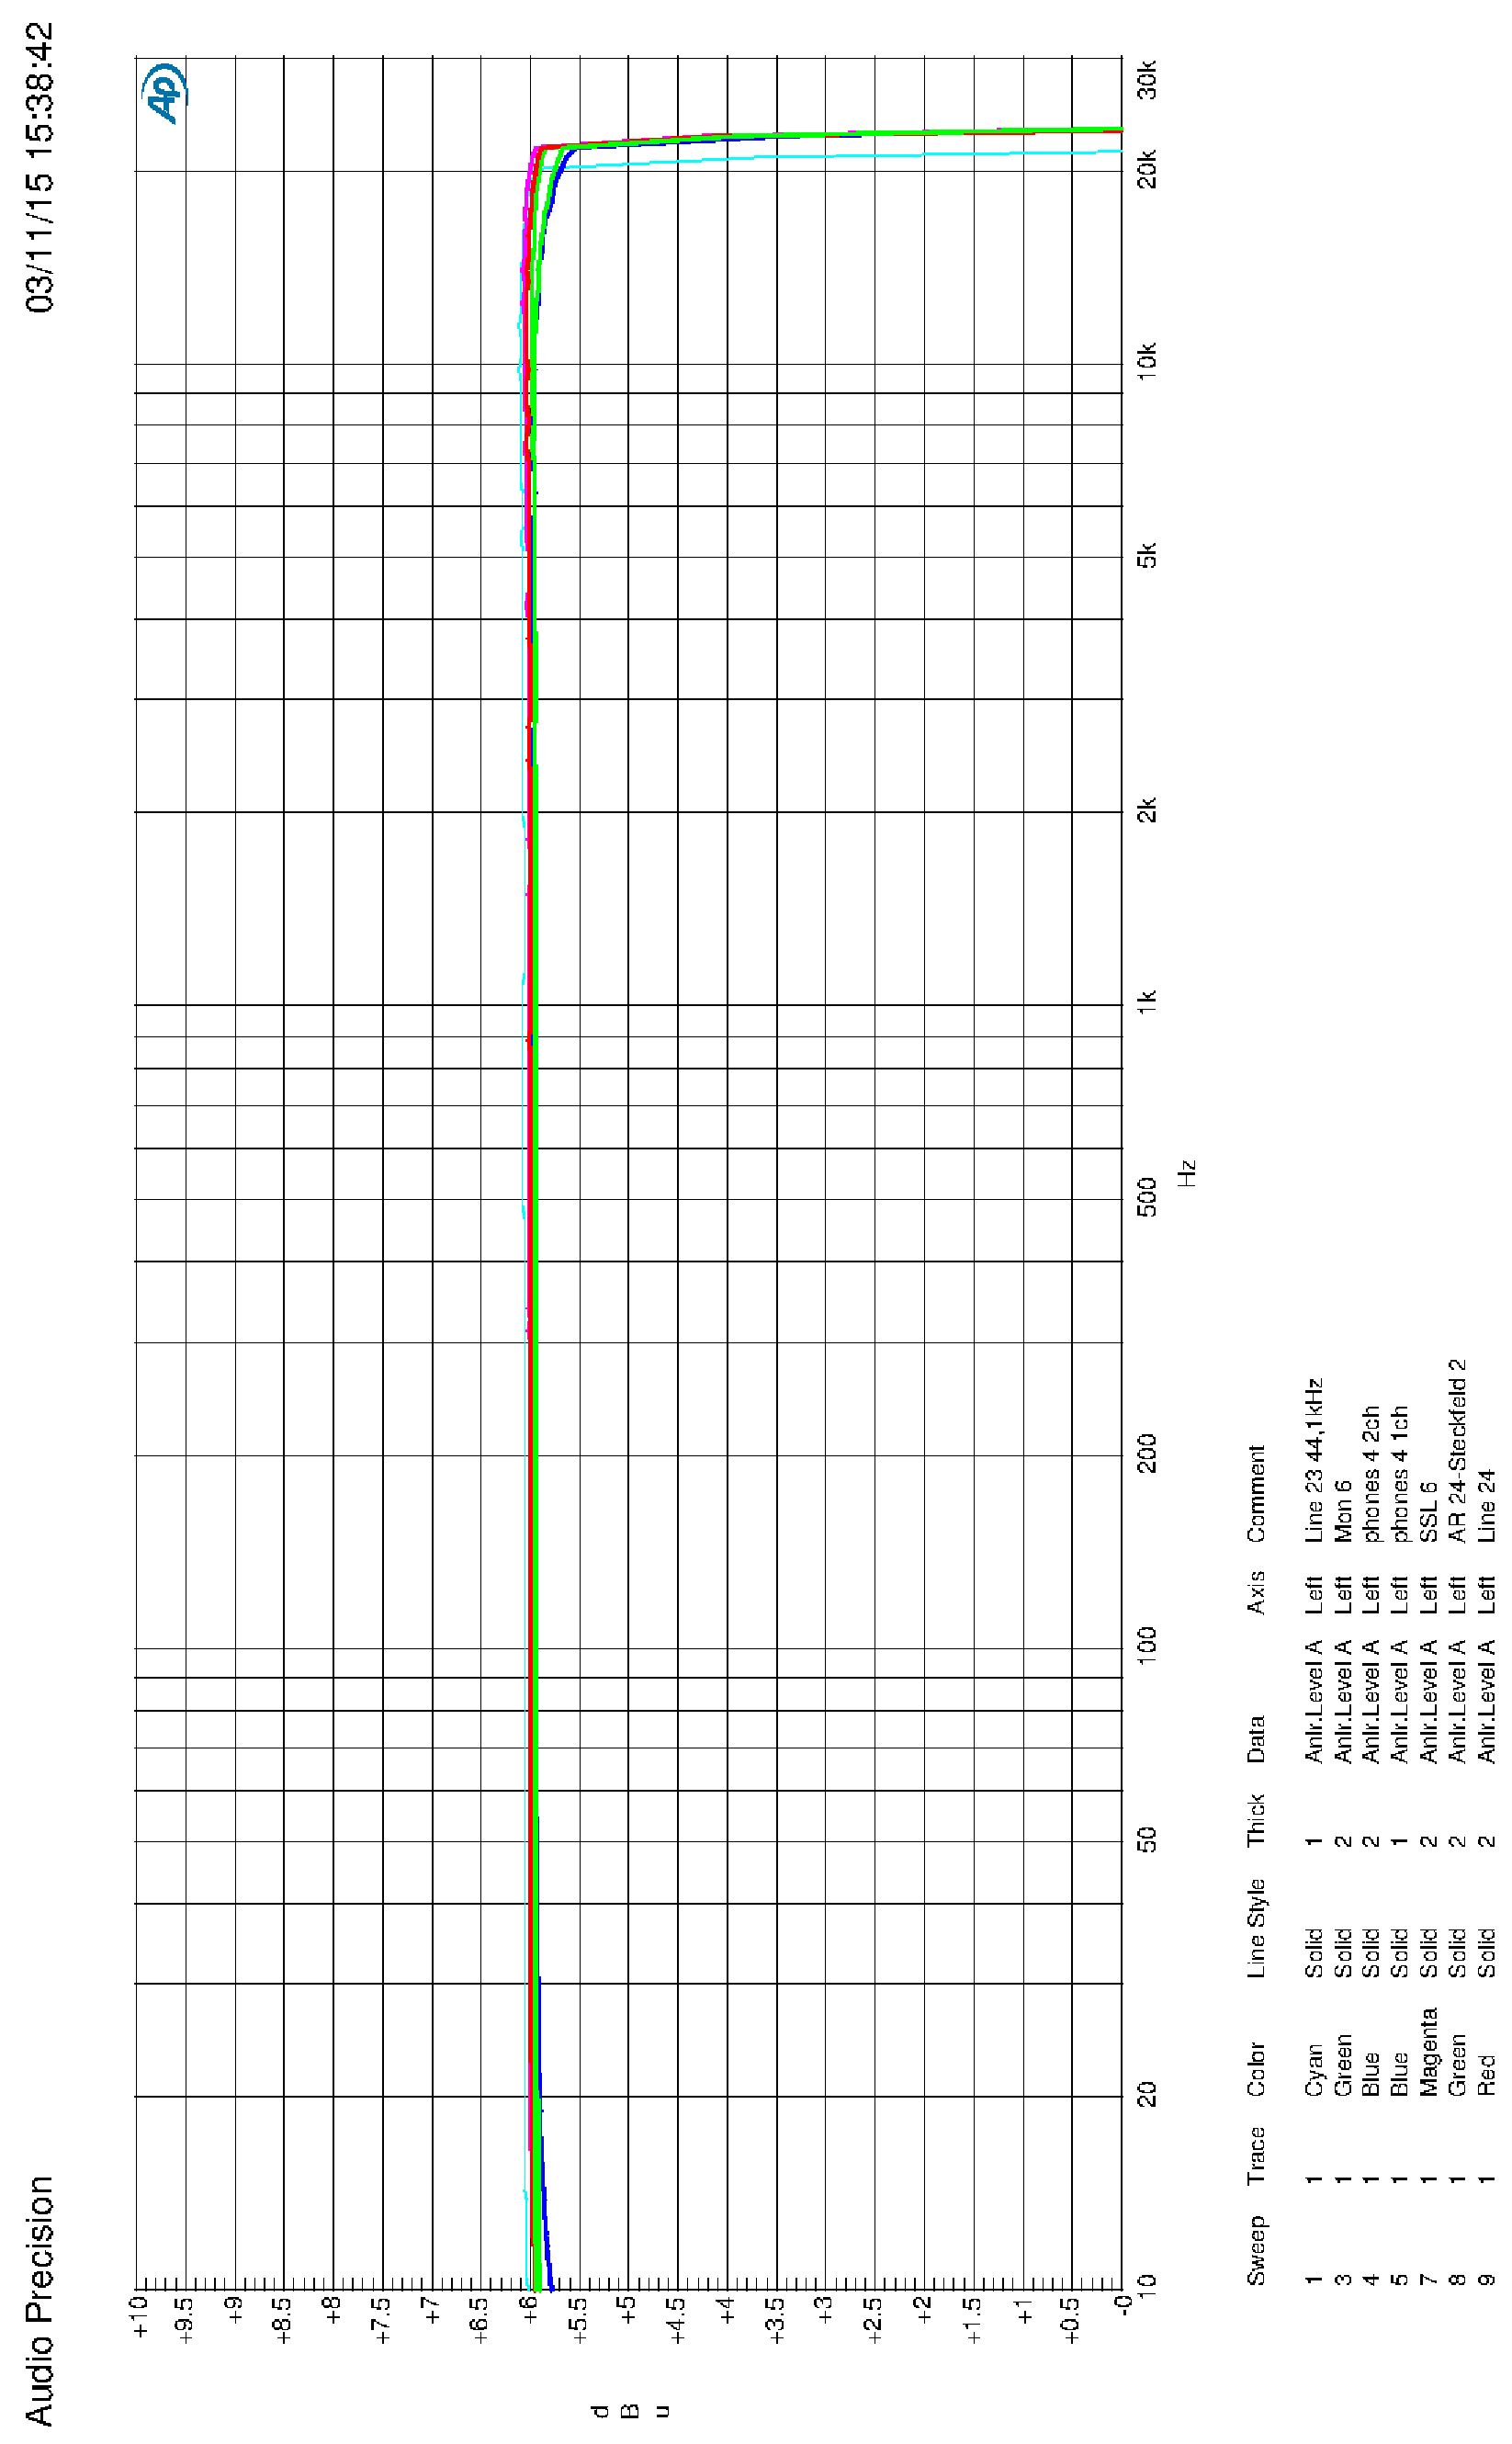
\includegraphics[width=14cm,keepaspectratio=true]{HQDAWandlerVergleich10dB}
\caption{frequency responses of different DACs (high resolution)}
\label{Abb.:1}
\end{center}
\end{figure}



\begin{figure}[htbp]
\begin{center}
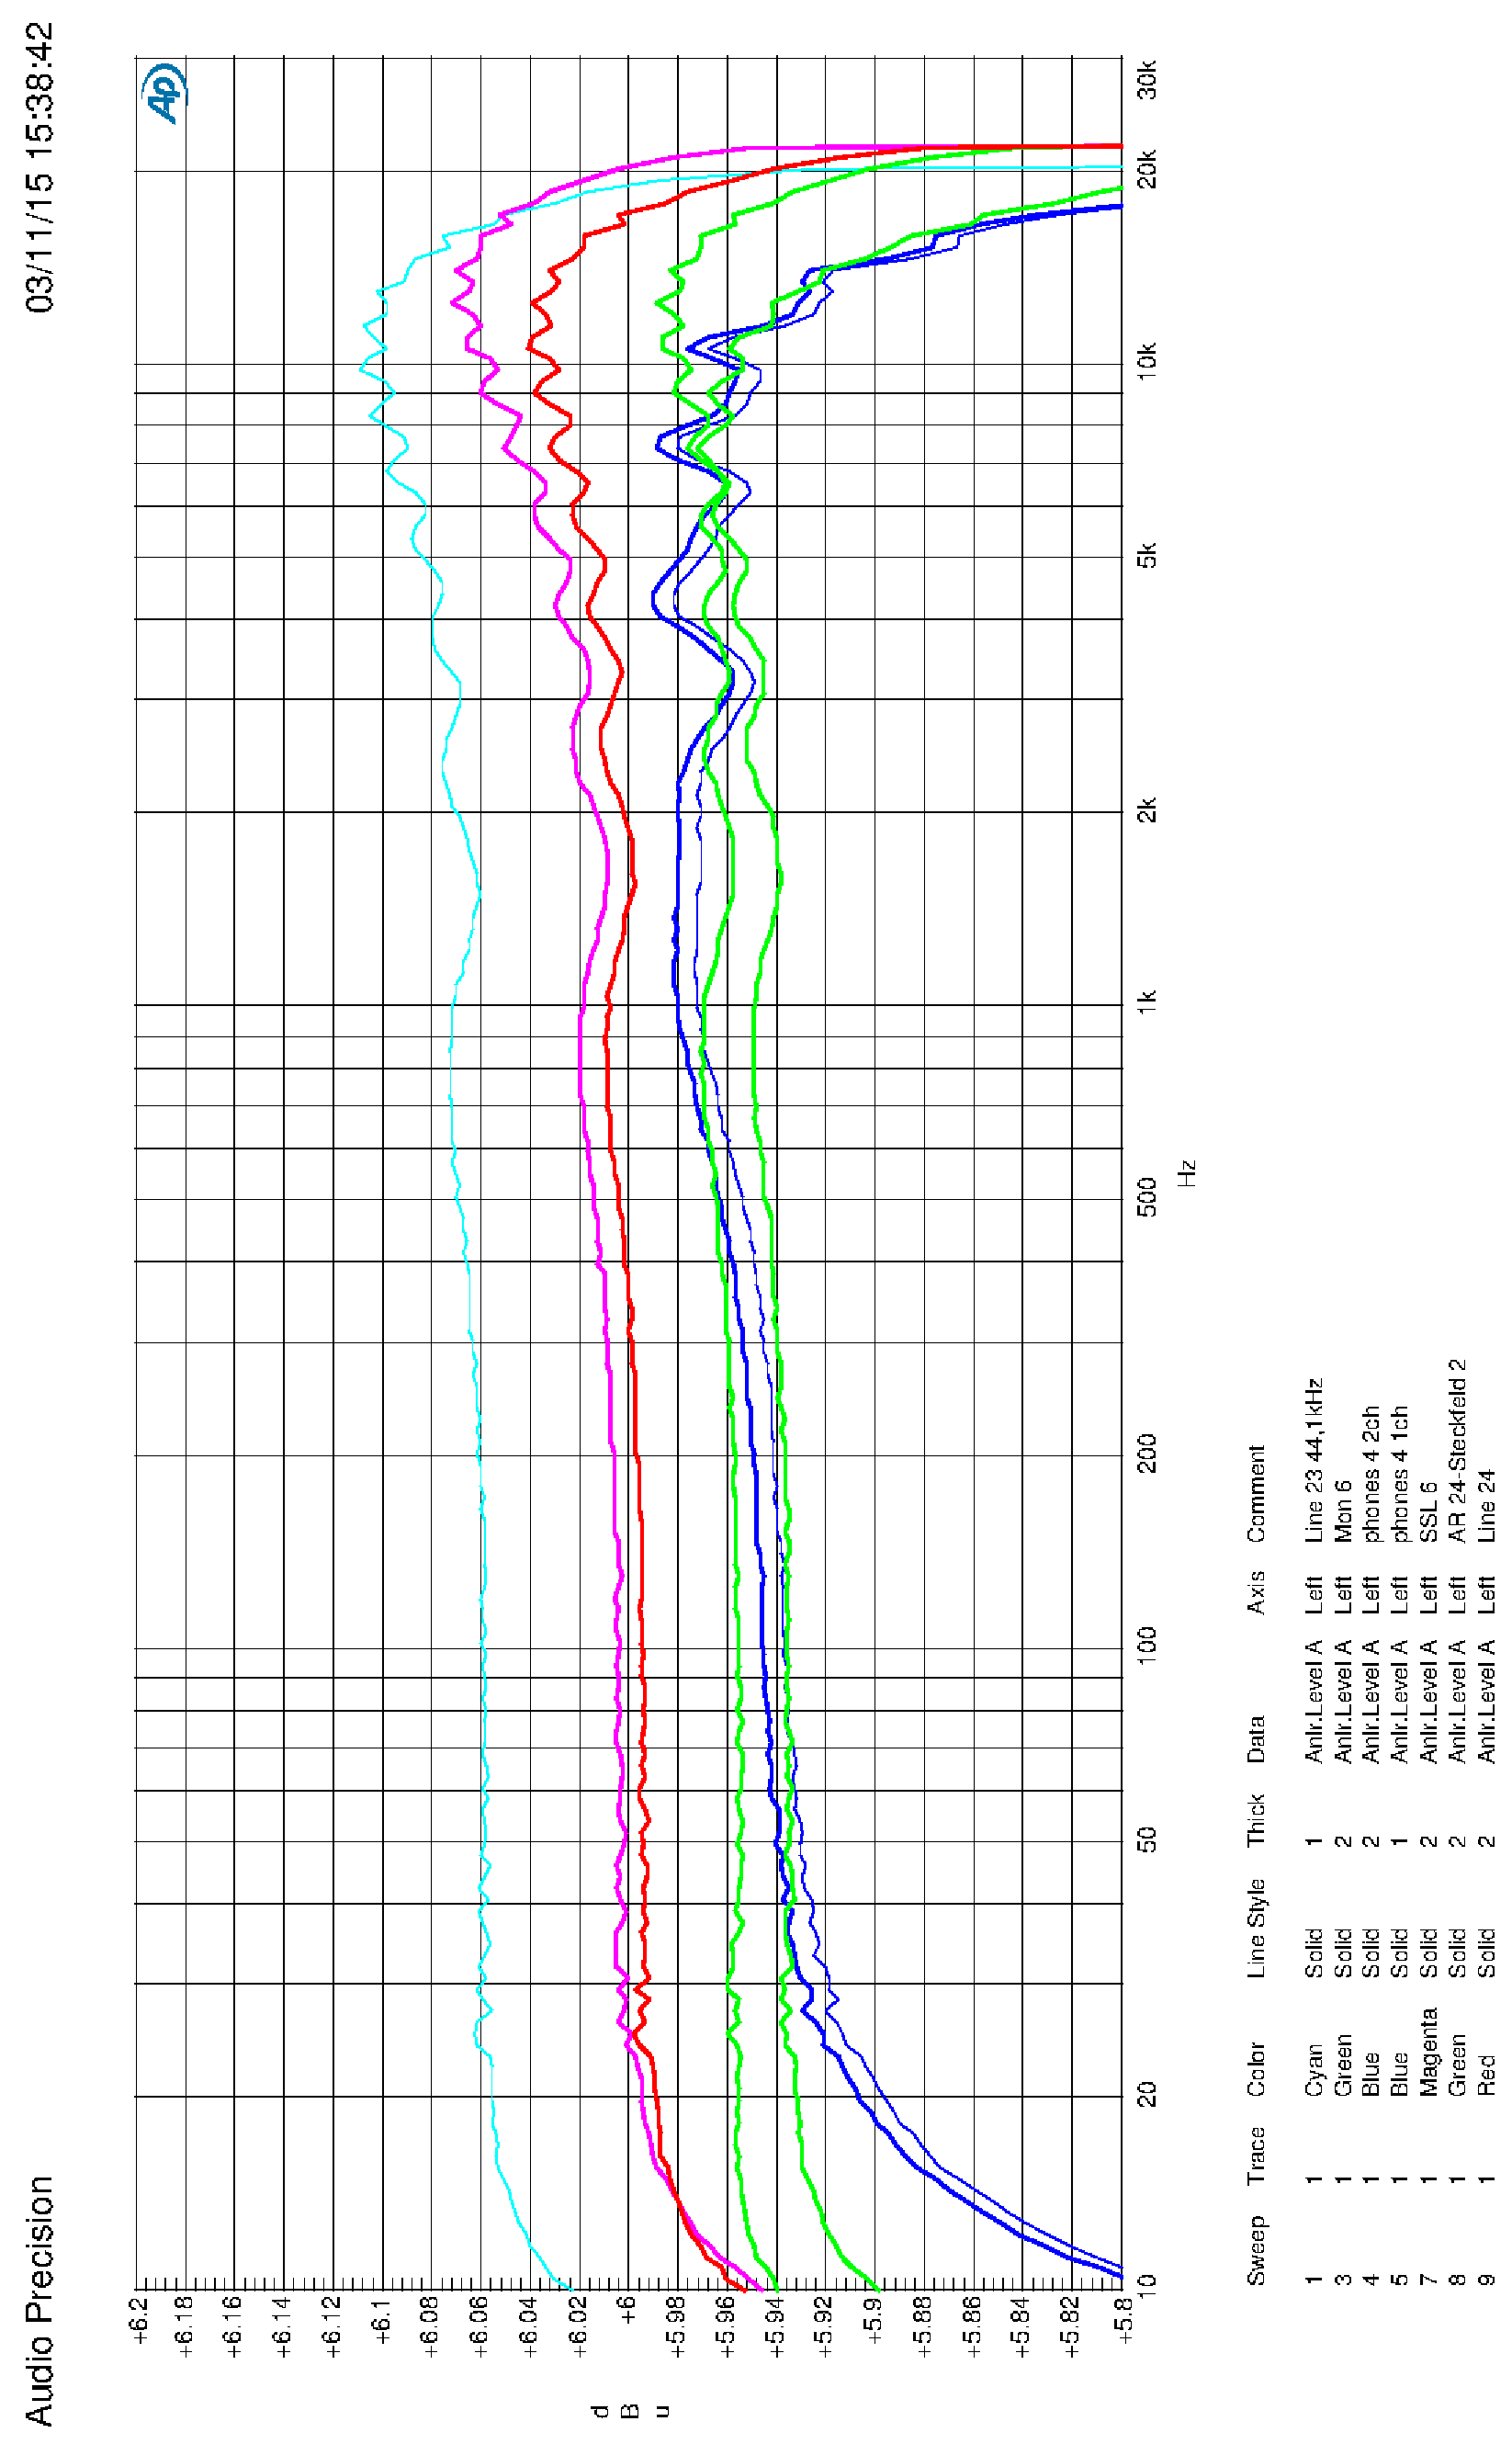
\includegraphics[width=14cm,keepaspectratio=true]{HQDaWandlerVergleich}
\caption{detailed frequency responses of different DACs (high resolution)}
\label{Abb.:1}
\end{center}
\end{figure}

\begin{figure}[htbp]
\begin{center}
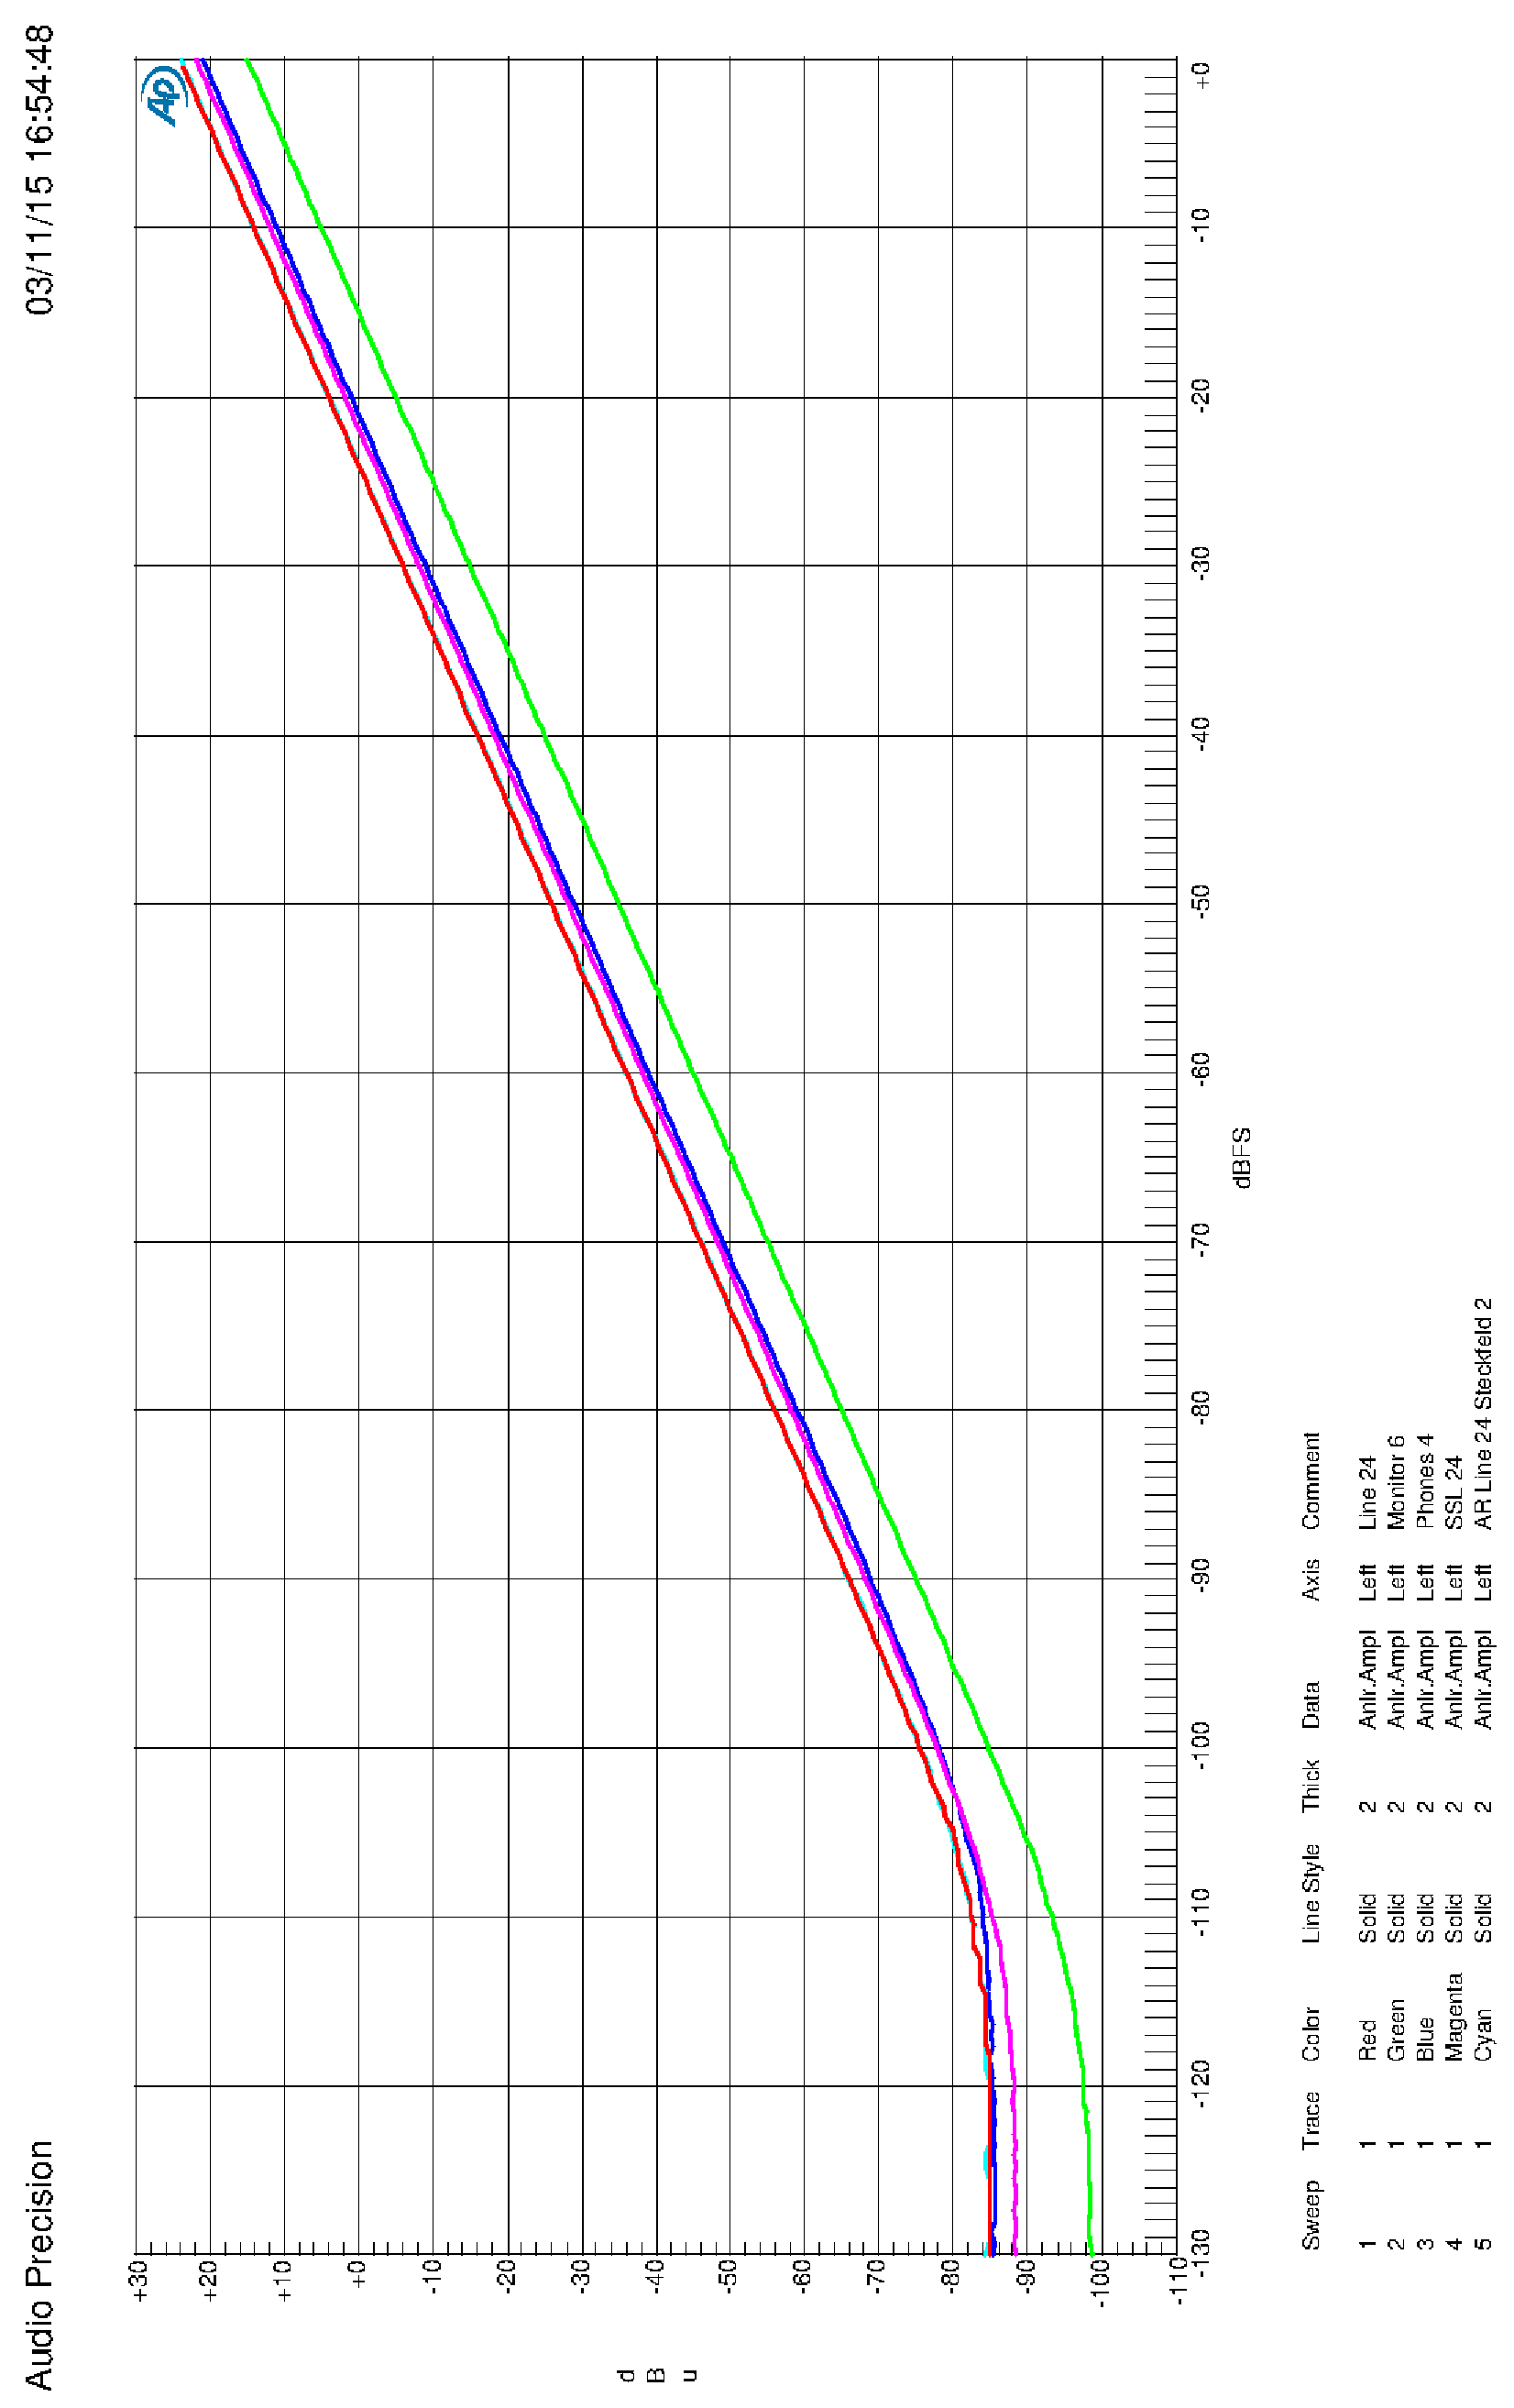
\includegraphics[width=14cm,keepaspectratio=true]{HQDynamikvergleich}
\caption{dynamic ranges of different DACs (high resolution)}
\label{Abb.:1}
\end{center}
\end{figure}

\begin{figure}[htbp]
\begin{center}
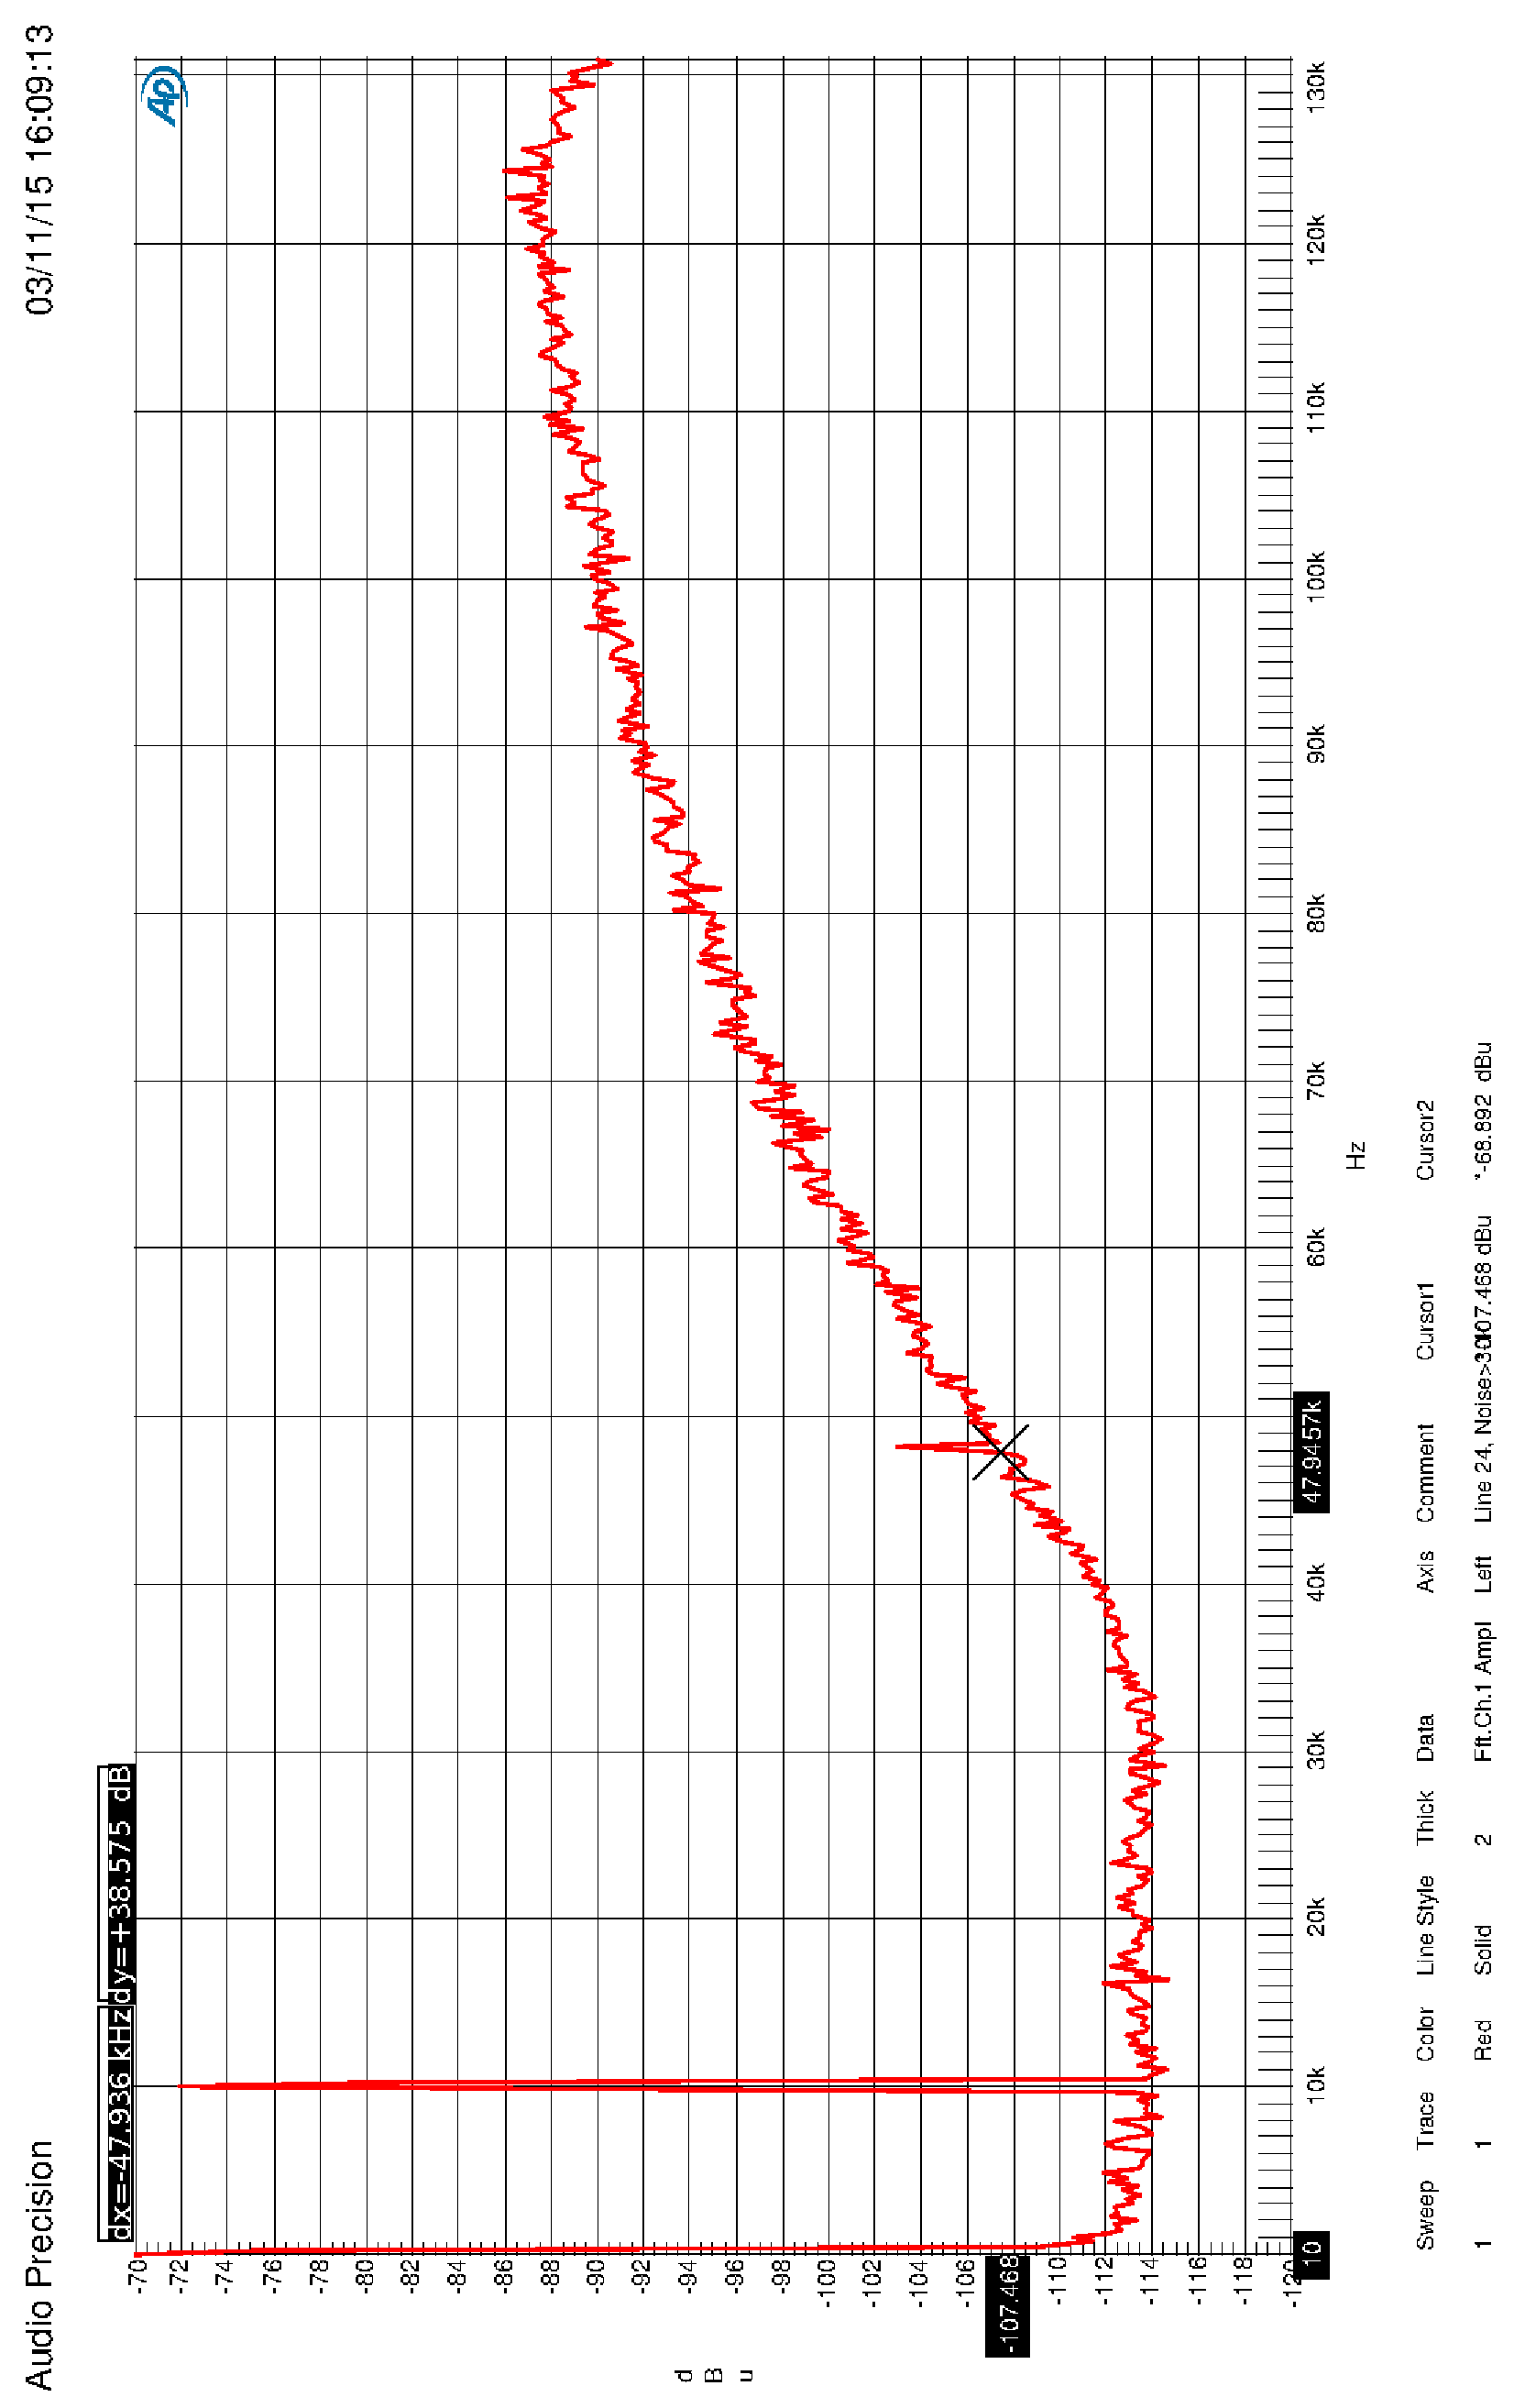
\includegraphics[width=14cm,keepaspectratio=true]{HQFFTrauschen}
\caption{FFT of line24 signal (high resolution)}
\label{Abb.:1}
\end{center}
\end{figure}

\begin{figure}[htbp]
\begin{center}
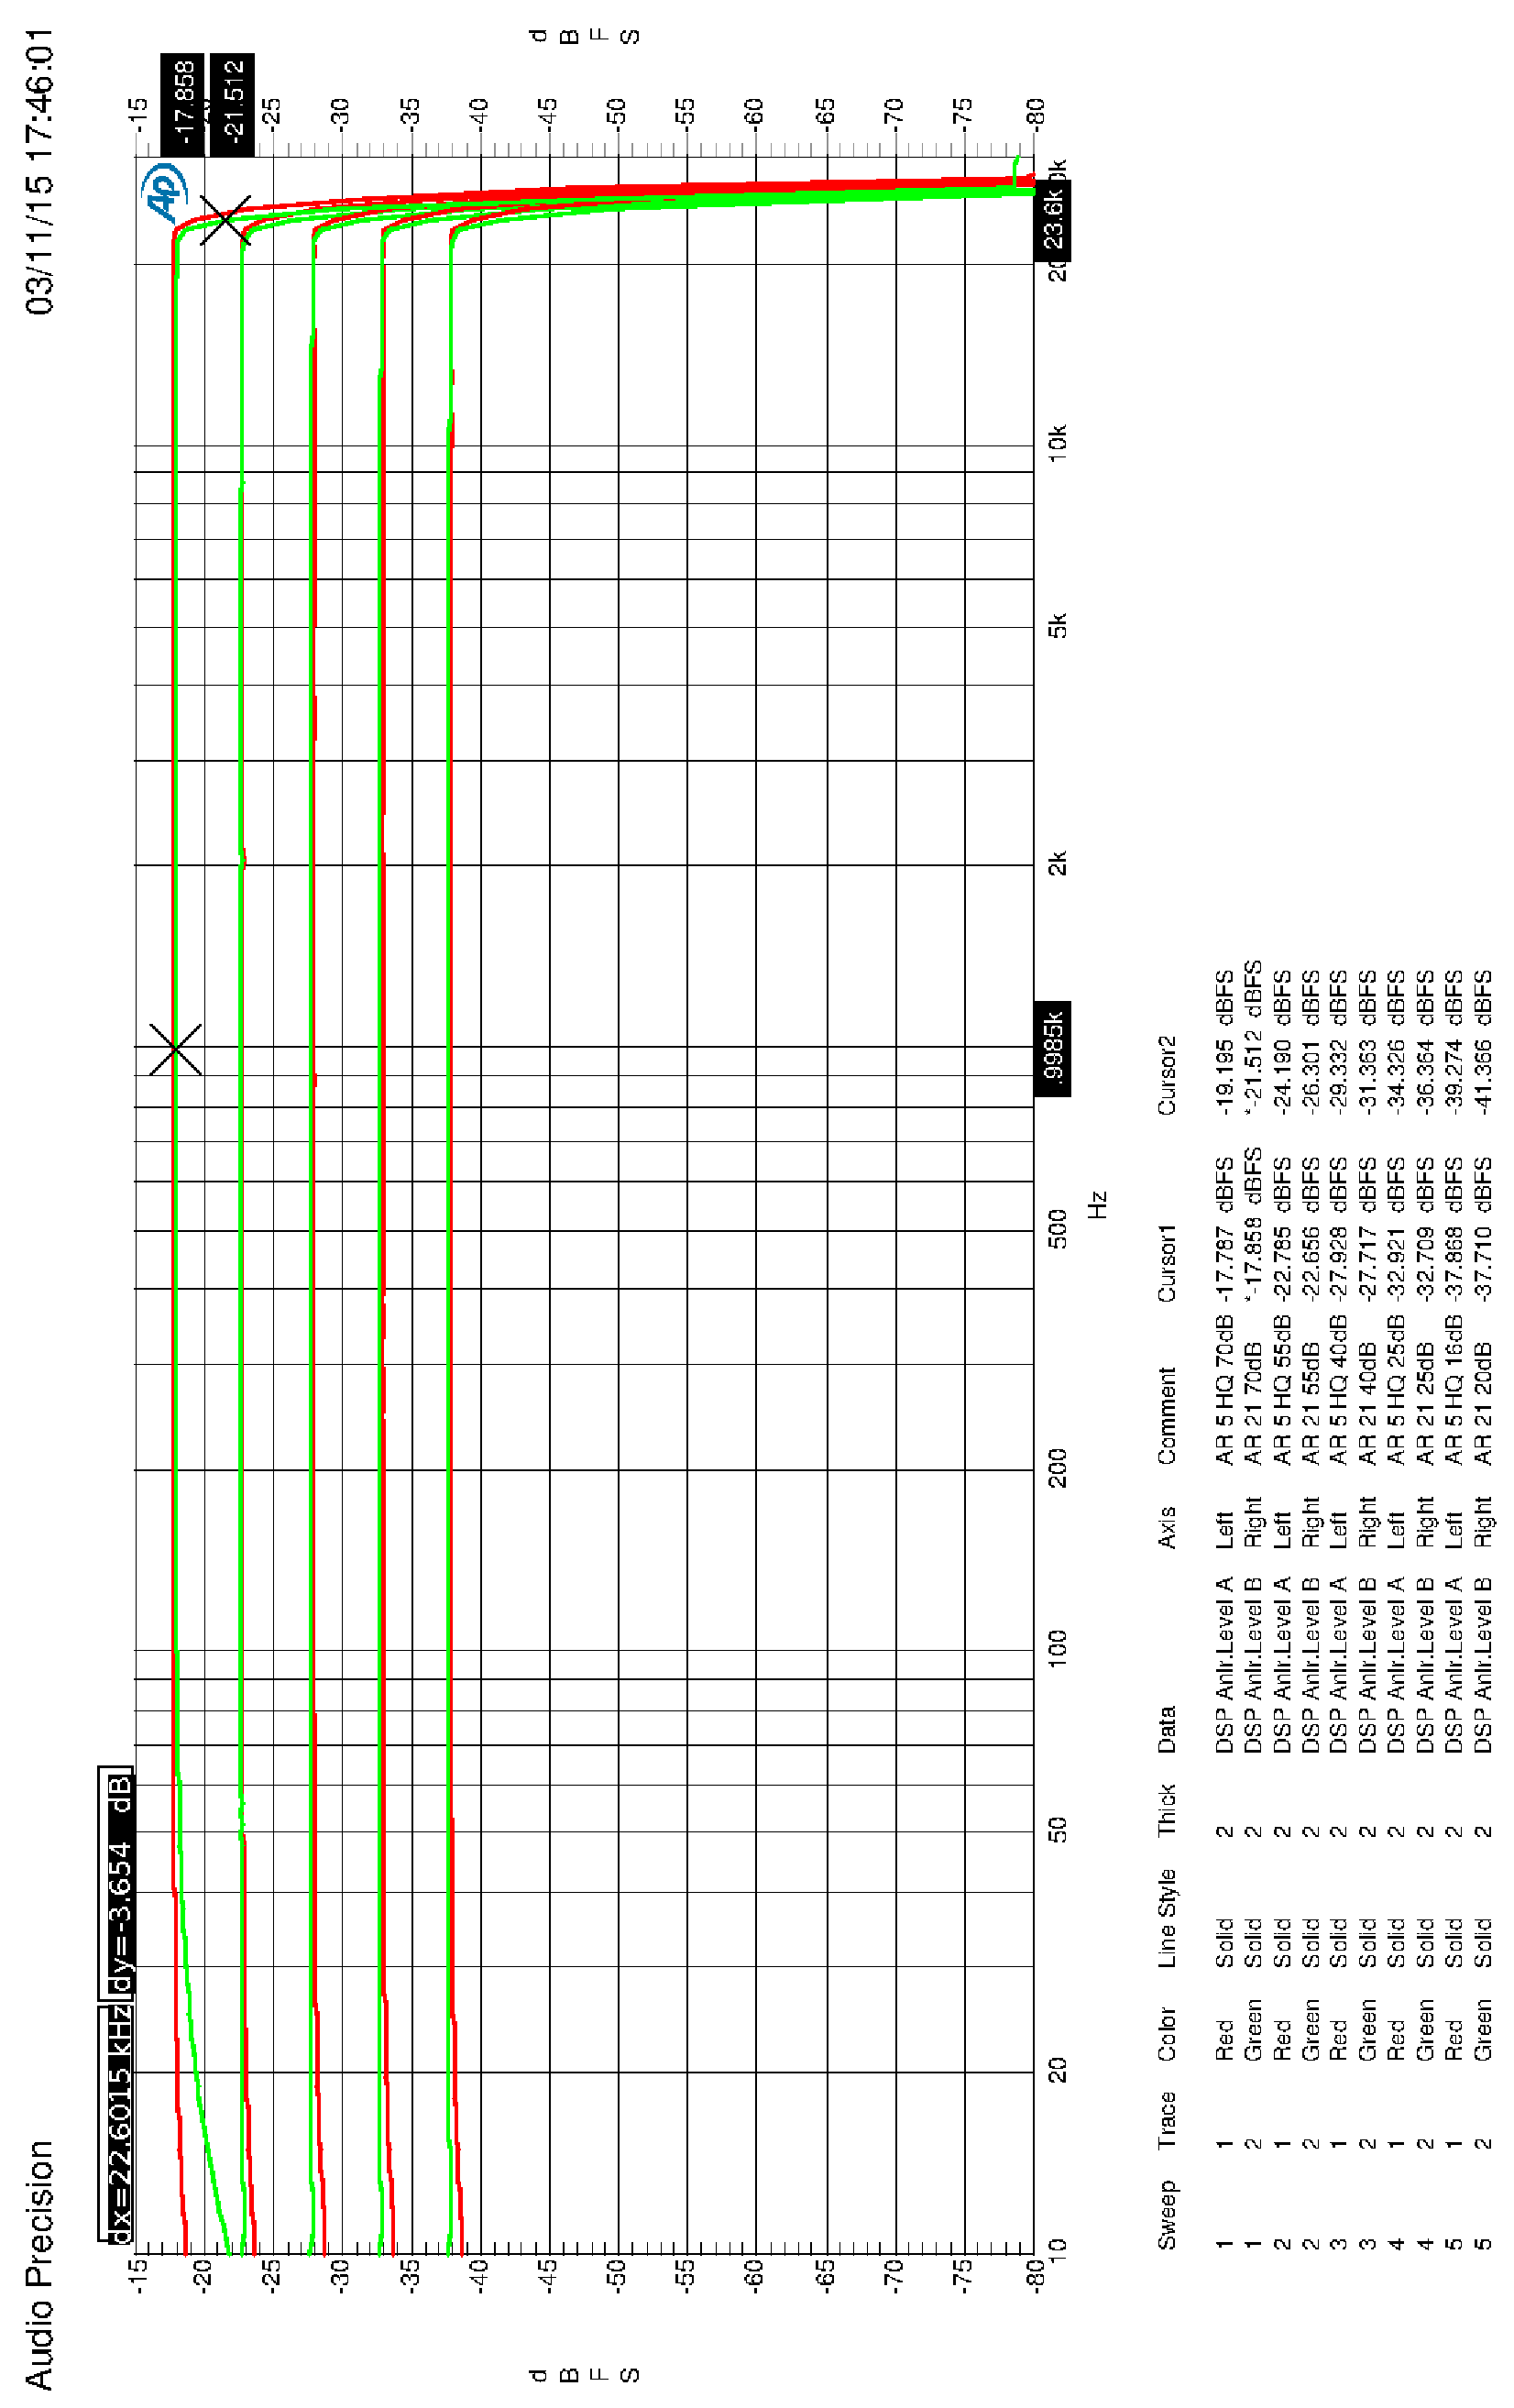
\includegraphics[width=14cm,keepaspectratio=true]{HQLAWOVorverstaerker5u21dB}
\caption{LAWO ADC and preamplifier (high resolution)}
\label{Abb.:1}
\end{center}
\end{figure}

\begin{figure}[htbp]
\begin{center}
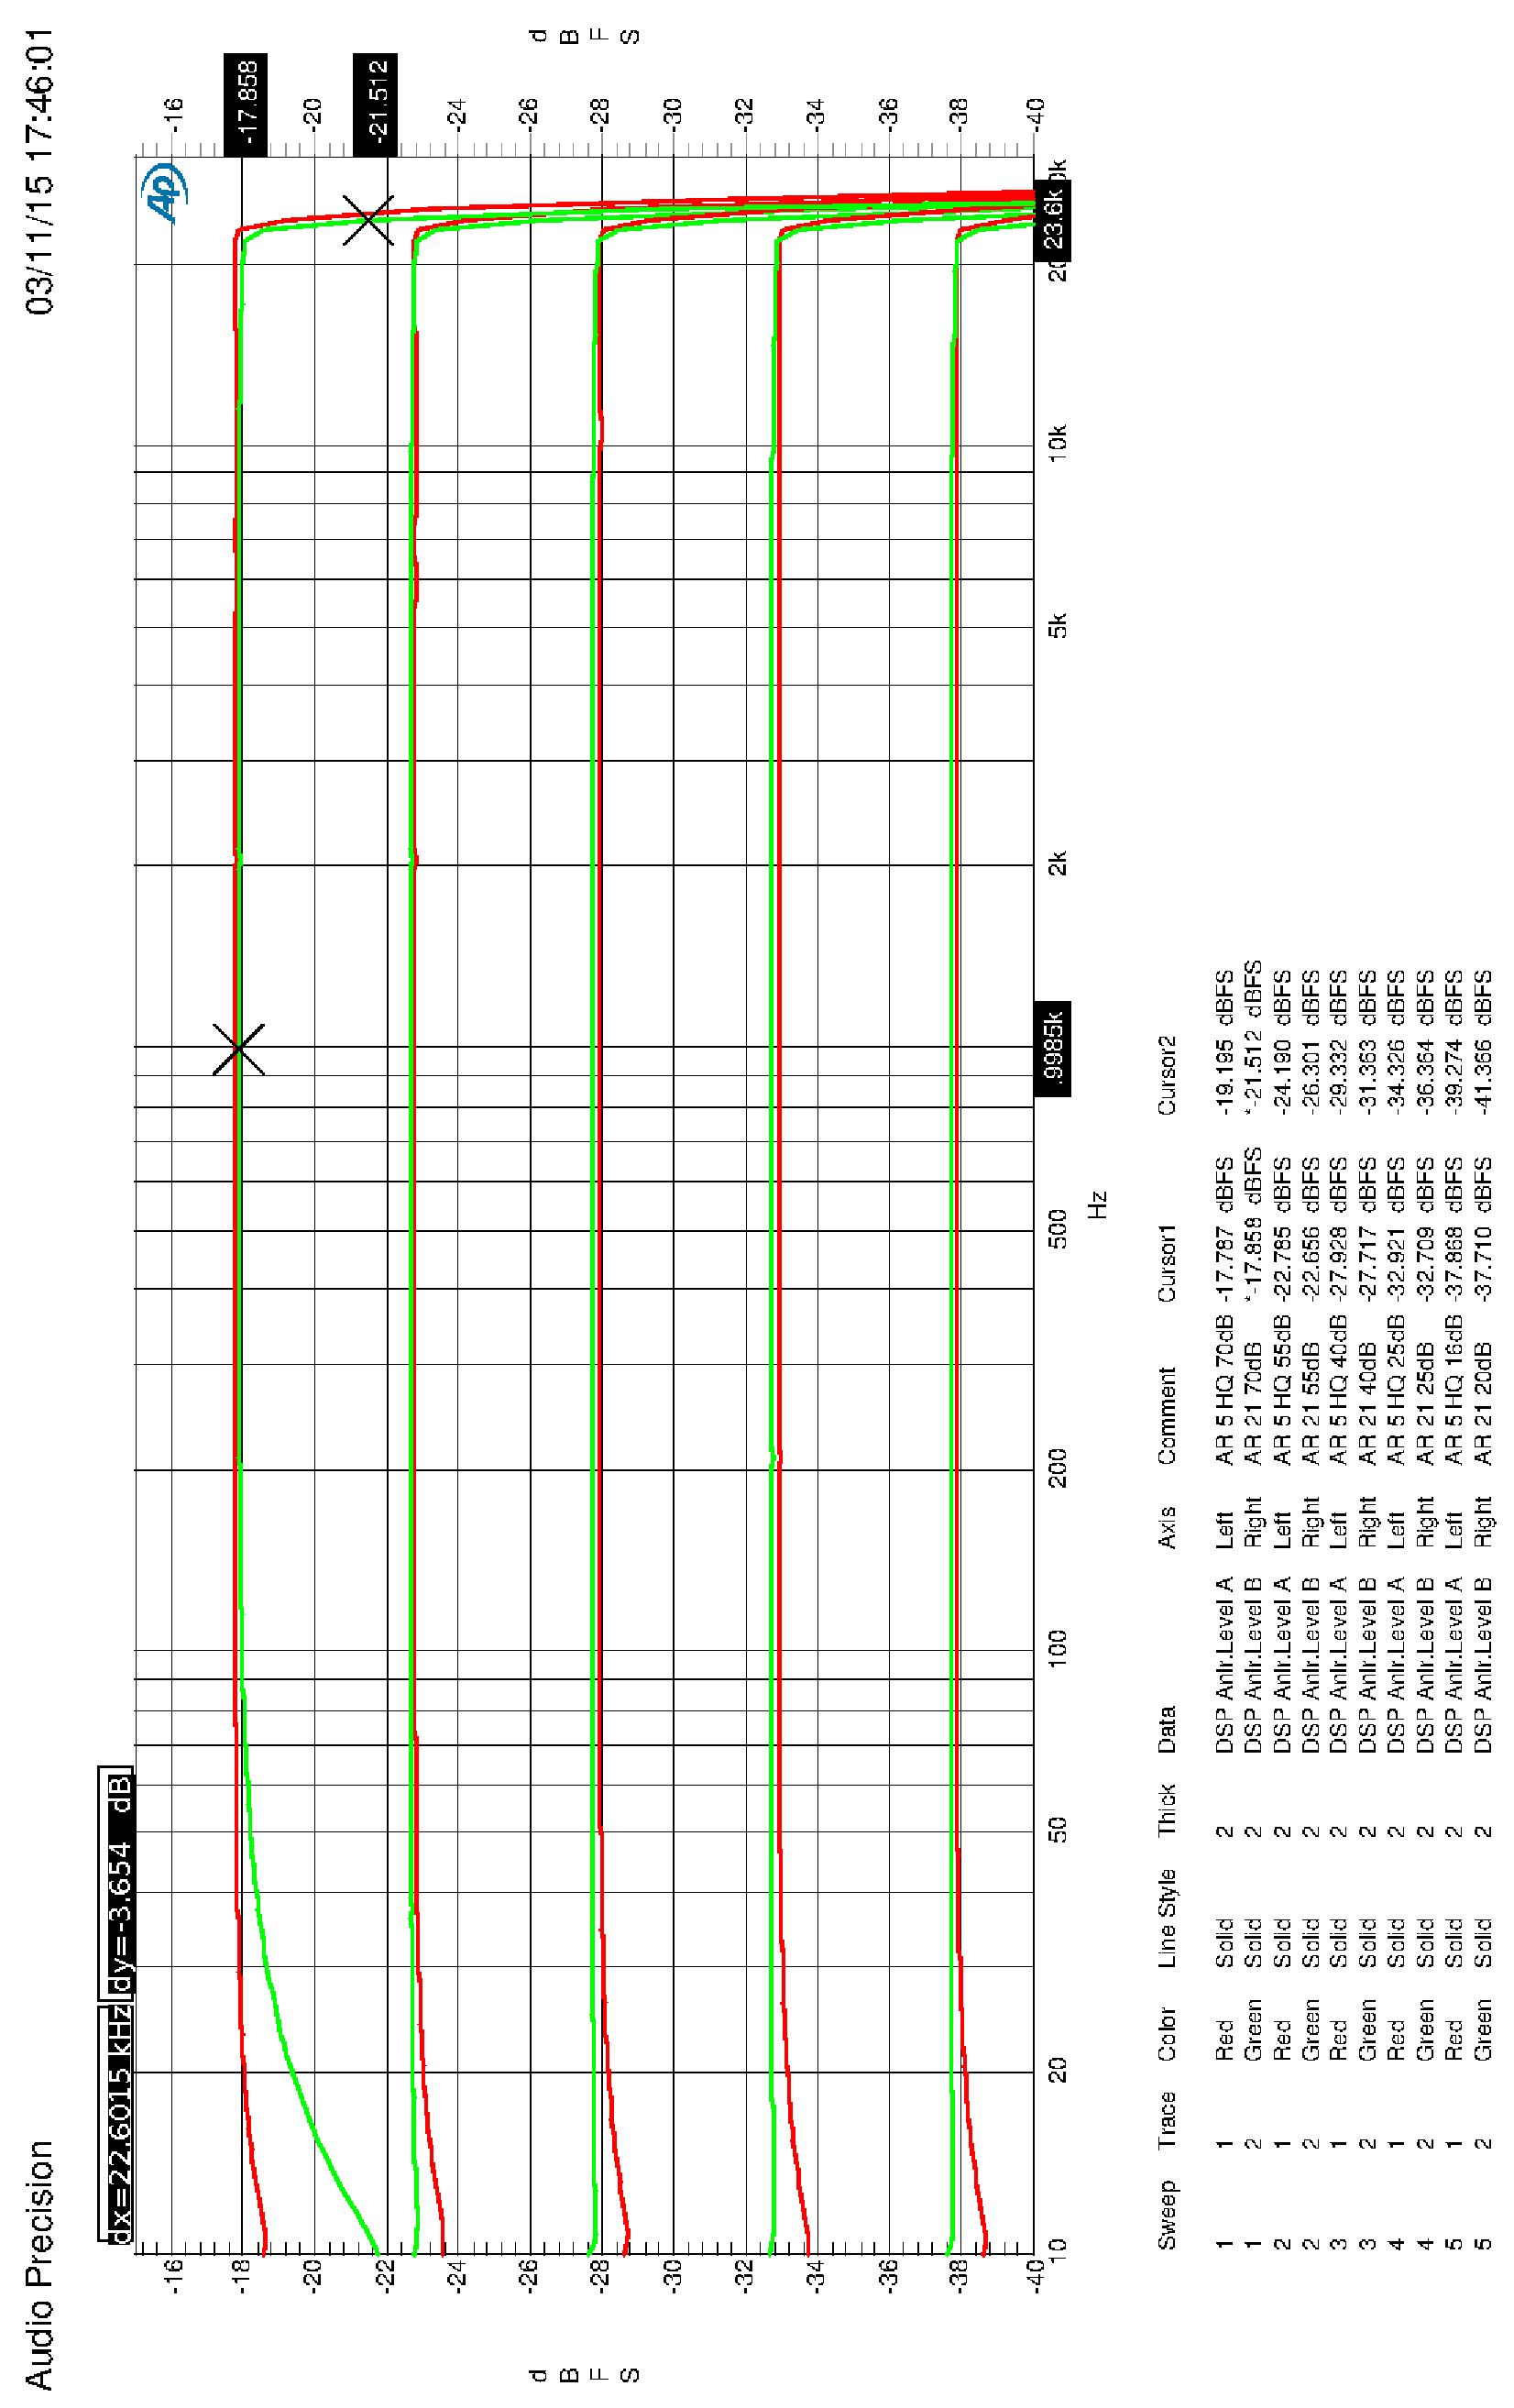
\includegraphics[width=14cm,keepaspectratio=true]{HQLAWOVorverstaerker5u21dBVergleichszoom}
\caption{LAWO ADC and preamplifier detailed view (high resolution)}
\label{Abb.:1}
\end{center}
\end{figure}

\begin{figure}[htbp]
\begin{center}
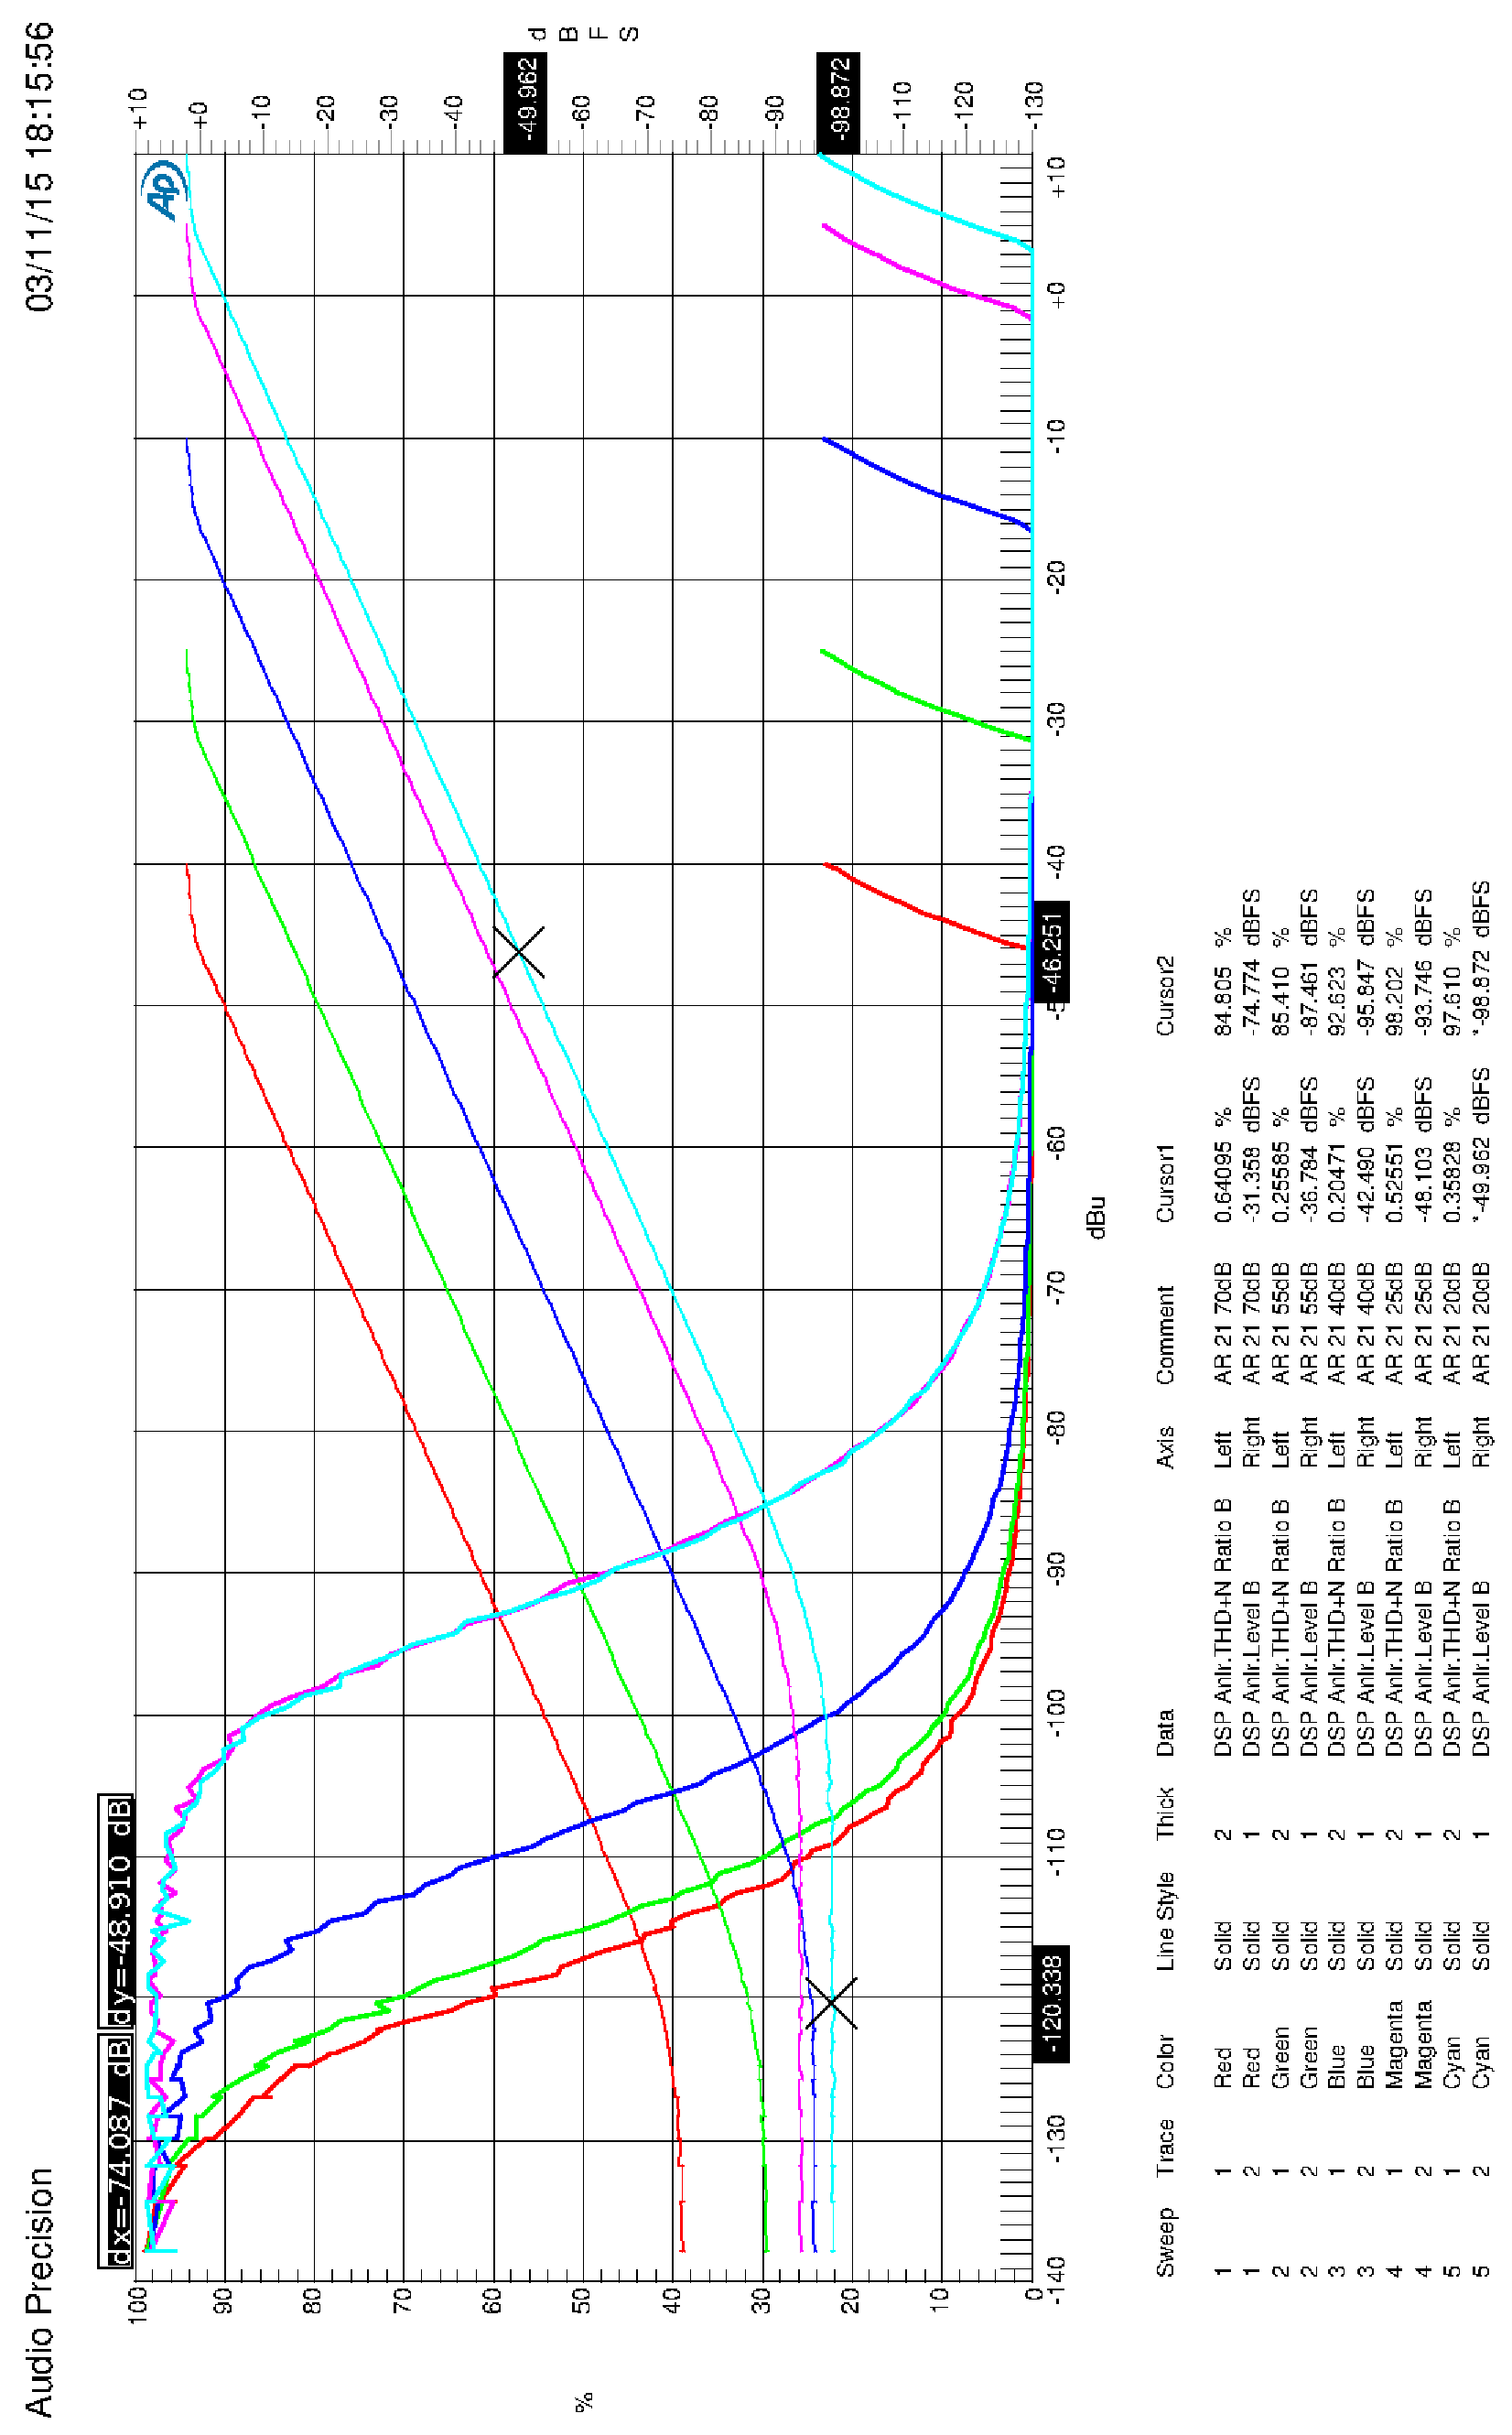
\includegraphics[width=14cm,keepaspectratio=true]{HQTHDAR21dBVergleich}
\caption{dynamic range of channel AR21 (high resolution)}
\label{Abb.:1}
\end{center}
\end{figure}

\begin{figure}[htbp]
\begin{center}
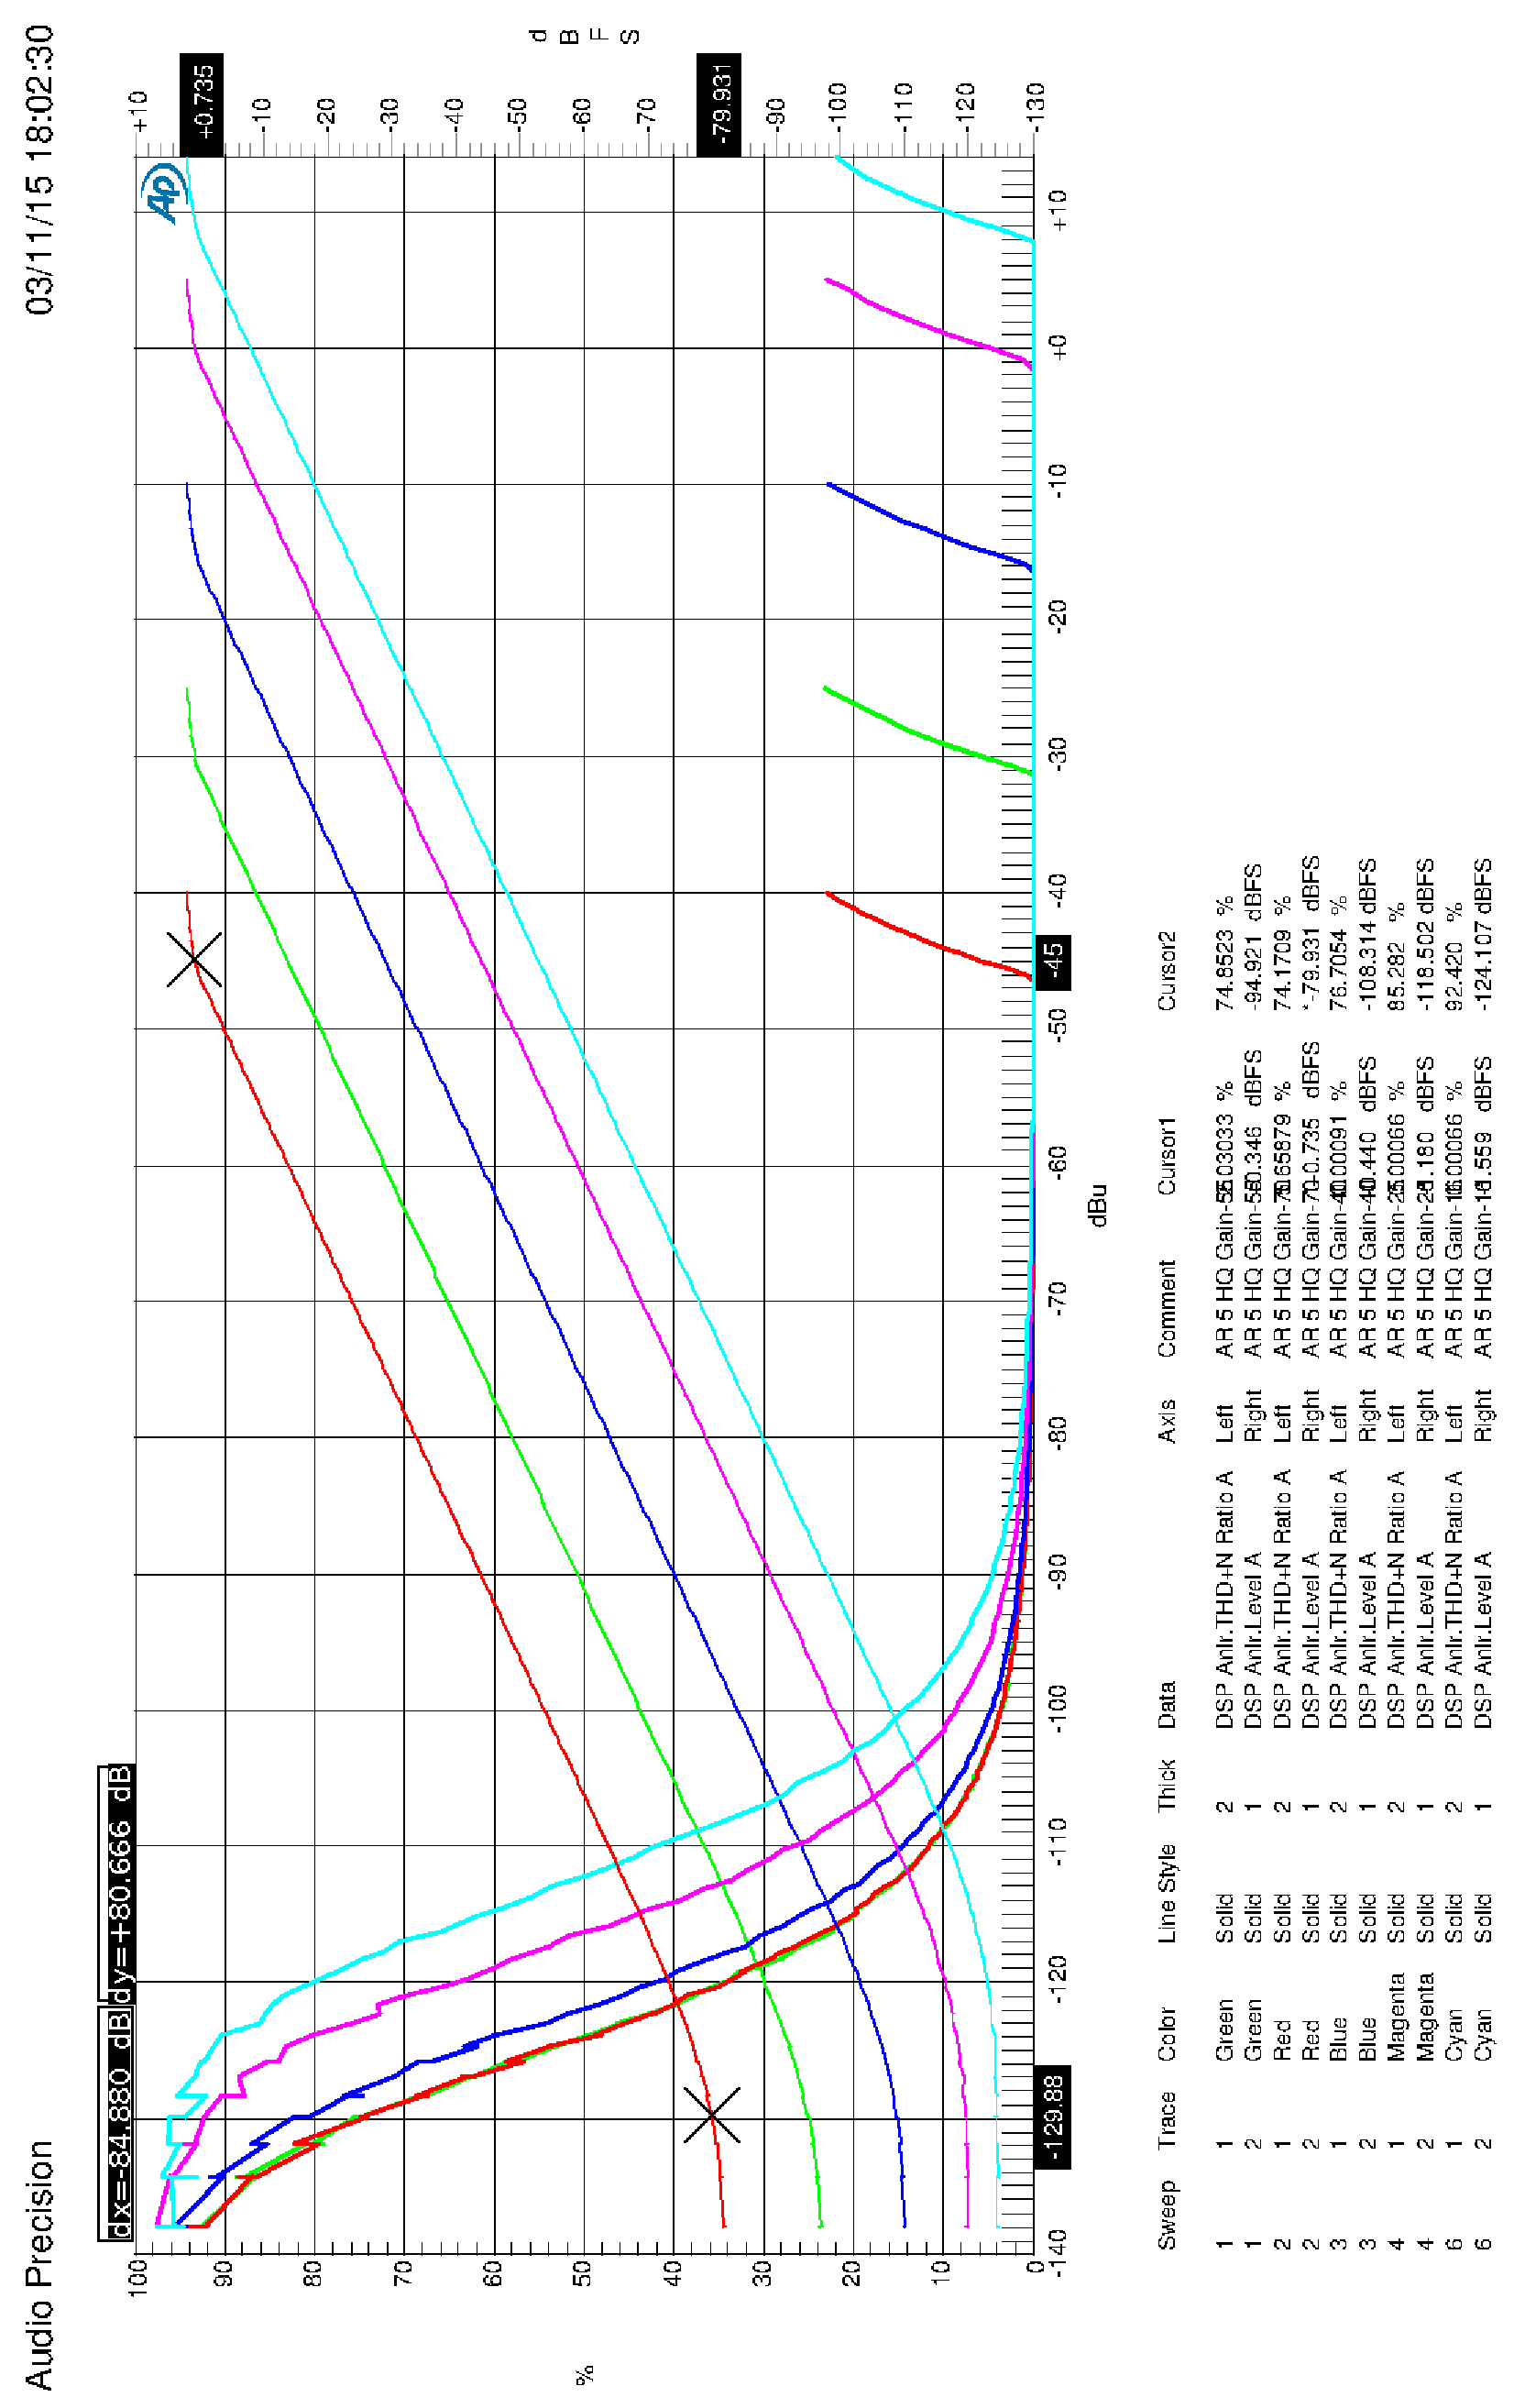
\includegraphics[width=14cm,keepaspectratio=true]{HQTHDAR5HQdBVergleich}
\caption{dynamic range of high quality channel AR5 (high resolution)}
\label{Abb.:1}
\end{center}
\end{figure}









\end{appendix}

%nicht referenzierte Literaturstellen

\nocite{mseifter88,pmandl97,weiss92,weiss92a,ginthoer93}

% Literaturverzeichnis einbinden, alpha, plain, unsrt, abbrv
\newpage
%Eintrag im Inhaltsverzeichnis
\addtocounter{page}{1}
\addcontentsline{toc}{chapter}{Literaturverzeichnis}
\addtocounter{page}{-1}

\bibliographystyle{alpha}

\bibliography{protokoll}

%Index File
%\input{diplom.ind}

\end{document}
